\documentclass[9pt,a4paper]{article}

% Basic packages
\usepackage[margin=1in]{geometry}
\usepackage{amsmath,amssymb,amsthm}
\usepackage{tikz}
\usetikzlibrary{arrows.meta,positioning,shapes,graphs,calc}
\usepackage{pgfplots}
\pgfplotsset{compat=1.17}
\usepackage{xcolor}
\usepackage{array}
\usepackage{tabularx}
\usepackage{hyperref}
\usepackage{microtype}
\usepackage{float}

% Unicode font support (required for Agda output - compile with lualatex)
\usepackage{fontspec}
\usepackage{unicode-math}

\setmainfont{DejaVu Serif}
\setsansfont{DejaVu Sans}
\setmonofont{DejaVu Sans Mono}[Scale=MatchLowercase]
\setmathfont{STIX Two Math}

% Agda literate support
\usepackage{agda}
\usepackage{agda-spec}

\renewcommand{\AgdaFontStyle}[1]{{\small\sffamily #1}}
\renewcommand{\AgdaKeywordFontStyle}[1]{{\small\sffamily\bfseries #1}}
\renewcommand{\AgdaBoundFontStyle}[1]{{\small\sffamily\itshape #1}}
\renewcommand{\AgdaStringFontStyle}[1]{{\small\ttfamily #1}}
\renewcommand{\AgdaCommentFontStyle}[1]{{\small\ttfamily #1}}

% Nord-inspired Agda colors
\definecolor{AgdaComment}      {HTML}{616E88}
\definecolor{AgdaPragma}       {HTML}{616E88}
\definecolor{AgdaKeyword}      {HTML}{5E81AC}
\definecolor{AgdaString}       {HTML}{A3BE8C}
\definecolor{AgdaNumber}       {HTML}{B48EAD}
\definecolor{AgdaSymbol}       {HTML}{4C566A}

\definecolor{AgdaBound}                 {HTML}{2E3440}
\definecolor{AgdaGeneralizable}         {HTML}{5E81AC}
\definecolor{AgdaInductiveConstructor}  {HTML}{8FBCBB}
\definecolor{AgdaCoinductiveConstructor}{HTML}{88C0D0}
\definecolor{AgdaDatatype}              {HTML}{81A1C1}
\definecolor{AgdaField}                 {HTML}{B48EAD}
\definecolor{AgdaFunction}              {HTML}{5E81AC}
\definecolor{AgdaMacro}                 {HTML}{A3BE8C}
\definecolor{AgdaModule}                {HTML}{E0BA62}
\definecolor{AgdaPostulate}             {HTML}{BF616A}
\definecolor{AgdaPrimitive}             {HTML}{81A1C1}
\definecolor{AgdaRecord}                {HTML}{81A1C1}
\definecolor{AgdaArgument}              {HTML}{4C566A}

\definecolor{nord0}{HTML}{2E3440}
\definecolor{nord1}{HTML}{3B4252}
\definecolor{nord2}{HTML}{434C5E}
\definecolor{nord3}{HTML}{4C566A}
\definecolor{nord4}{HTML}{D8DEE9}
\definecolor{nord5}{HTML}{E5E9F0}
\definecolor{nord6}{HTML}{ECEFF4}
\definecolor{nord7}{HTML}{8FBCBB}
\definecolor{nord8}{HTML}{88C0D0}
\definecolor{nord9}{HTML}{81A1C1}
\definecolor{nord10}{HTML}{5E81AC}
\definecolor{nord11}{HTML}{BF616A}
\definecolor{nord12}{HTML}{D08770}
\definecolor{nord13}{HTML}{EBCB8B}
\definecolor{nord14}{HTML}{A3BE8C}
\definecolor{nord15}{HTML}{B48EAD}

\urlstyle{tt}
\newcommand{\fpath}[1]{\nolinkurl{#1}}

\theoremstyle{plain}
\newtheorem{theorem}{Theorem}
\newtheorem{lemma}[theorem]{Lemma}
\newtheorem{corollary}[theorem]{Corollary}
\theoremstyle{definition}
\newtheorem{definition}{Definition}
\theoremstyle{remark}
\newtheorem{remark}{Remark}

\title{\textbf{Coinductive Homomorphism Reinforcement Learning} \\
Optimality as Structure Preservation}

\author{Ricardo Corral-Corral}
\date{April 2026}

\begin{document}

\maketitle

\begin{abstract}
Traditional reinforcement learning defines optimality by maximizing a scalar return---a criterion that collapses infinite reward sequences into a single number, discarding their temporal structure.
We propose a different foundation: an action is optimal when it leads to a state from which the agent's future is best.

What makes one state better than another?
Acting optimally from it yields higher rewards at every future depth.
And what makes \emph{those} rewards higher?
The states reachable from there are themselves better---by the same criterion, unfolding without bound.
This coinductive structure is the core of our definition: a \textbf{coinductive homomorphism} is an action ranking that preserves the quality ordering on the states actions lead to.

The definition is an order homomorphism from action rankings into a coinductively ordered codomain, and it decouples optimality from immediate transition rewards.
An action that sacrifices immediate reward to reach a superior state is correctly ranked---a pattern that arises naturally in investment, exploration, and preparation.

A natural strengthening additionally requires that immediate transition rewards respect the ranking, bundling two orthogonal conditions into a single requirement on the full action-value stream.
We prove that the two conditions decompose cleanly, that the coinductive homomorphism alone is strictly more general, and that the top-ranked action maximizes cumulative return from successor states at every finite horizon.
Three verified environments of increasing structural complexity demonstrate settings where the coinductive homomorphism correctly ranks actions but its action-value strengthening cannot.

We prove seven main results, all machine-verified in Agda:
\textbf{(1)}~Subsumption: both conditions imply classical argmax optimality for any finite horizon;
\textbf{(2)}~Monotonic learning: ranking updates via violation-correction converge in at most $|S| \cdot \binom{|A|}{2}$ swaps;
\textbf{(3)}~Instant adaptation: when actions become unavailable, the next-best action is $O(1)$ lookup;
\textbf{(4)}~Stochastic extension: the framework lifts to probabilistic environments via the Giry monad, where rankings preserve lexicographic expected stream dominance;
\textbf{(5)}~Distributional hierarchy: FOSD and the SD$[k]$ chain give parameterized verification strength for broader utility classes;
\textbf{(6)}~Compositional algebra: verified rankings compose via product, sum, convolution, and scaling;
\textbf{(7)}~State abstraction: rankings verified on finite abstract systems lift to arbitrary concrete state spaces;
\textbf{(8)}~Scalable verification: a modular Environment Class architecture provides automatic trace-to-stream bridges, demonstrated with a full coinductive homomorphism for $8$-Queens ($8^8$ search space, zero postulates).

This document is itself the proof: compiling it with \texttt{agda --latex} type-checks all embedded code while producing this PDF.
\end{abstract}

%%%%%%%%%%%%%%%%%%%%%%%%%%%%%%%%%%%%%%%%%%%%%%%%%%%%%%%%%%%%%%%%%%%%%%%%%%%%%%%
% PART I: MOTIVATION
%%%%%%%%%%%%%%%%%%%%%%%%%%%%%%%%%%%%%%%%%%%%%%%%%%%%%%%%%%%%%%%%%%%%%%%%%%%%%%%

\section{Motivation: The Limitations of Scalar Returns}

Reinforcement learning (RL) studies agents that learn to make sequential decisions by interacting with an environment~\cite{Sutton2018}.  At each discrete time step, the agent observes a \emph{state}, selects an \emph{action}, and receives a numerical \emph{reward} that signals how good the outcome was.  The agent's goal is to find a \emph{policy}---a rule mapping states to actions---that collects as much reward as possible over time.

The question is how to define ``as much reward as possible.''  The dominant answer in modern RL is the \emph{expected discounted return}: given a policy~$\pi$, the agent averages over all trajectories~$\tau$ it might experience:
\[
J(\pi) = \mathbb{E}_{\tau \sim \pi} \left[ \sum_{t=0}^{\infty} \gamma^t r_t \right]
\]
where $r_t$ is the reward at time~$t$ and $\gamma \in [0,1)$ is the \emph{discount factor}.  The discount makes future rewards exponentially less valuable: a reward 10~steps ahead counts for only~$\gamma^{10}$ of its face value.  This ensures the sum converges and makes the problem mathematically tractable.

The result is a single scalar.  A policy is optimal when it maximizes this number.  This formulation---rooted in Bellman's dynamic programming principle \cite{Bellman1957} and operationalized by algorithms like Q-learning \cite{Watkins1992}, policy gradient methods, and deep RL \cite{Mnih2015}---has driven remarkable successes, from game playing to robotics.

\subsection{The Problem: Temporal Structure Loss}

The difficulty is that this scalar discards the \emph{temporal structure} of the reward sequence.  Consider two futures:

\begin{center}
\begin{tabular}{lcc}
\textbf{Future} & \textbf{Reward Sequence} & \textbf{Sum ($\gamma{=}0.9$)} \\
\hline
A: ``Win then die'' & $[10, -5, 0, 0, \ldots]$ & $10 - 4.5 = 5.5$ \\
B: ``Struggle then thrive'' & $[0, 5, 0, 0, \ldots]$ & $0 + 4.5 = 4.5$ \\
\end{tabular}
\end{center}

A scalar optimizer chooses Future~A.  But \emph{structurally}, Future~B may be preferable---it avoids catastrophic failure and enters a productive state.  The sum erases this distinction.  This is \textbf{value aliasing}: structurally different futures mapping to the same scalar.

The problem deepens with several well-known artifacts of scalar aggregation:
\begin{itemize}
\item \textbf{The Discount Factor ($\gamma$):} An extrinsic parameter that controls how quickly future rewards are attenuated.  It systematically undervalues delayed payoffs, making the agent short-sighted by design.  No single $\gamma$ is correct for all environments, yet the optimal policy can change discontinuously as $\gamma$ varies.
\item \textbf{Instability:} Q-learning bootstraps scalar estimates of $J(\pi)$, leading to the deadly triad of function approximation, bootstrapping, and off-policy learning \cite{Sutton2018}.
\item \textbf{Credit Assignment:} A reward at $t{=}1000$ is discounted by $\gamma^{1000} \approx 0$, making long-horizon learning effectively impossible under standard discounting.
\end{itemize}

\noindent These are not implementation bugs---they are consequences of the scalar return formulation itself.  When the best course of action requires accepting a cost now in exchange for a benefit later, discounting can make the sacrifice appear irrational.

\subsection{Our Approach}

We propose to define optimality via \emph{structure preservation} rather than scalar maximization.  Instead of compressing the reward sequence into a number, we keep it as an infinite stream and define action rankings that preserve the quality ordering of successor states at every depth.  The question is: what structure should be preserved, and how?

%%%%%%%%%%%%%%%%%%%%%%%%%%%%%%%%%%%%%%%%%%%%%%%%%%%%%%%%%%%%%%%%%%%%%%%%%%%%%%%
% PART II: THE IDEA
%%%%%%%%%%%%%%%%%%%%%%%%%%%%%%%%%%%%%%%%%%%%%%%%%%%%%%%%%%%%%%%%%%%%%%%%%%%%%%%

\section{Structural Optimality: Successor State Quality}\label{sec:key-idea}

Consider an agent choosing between two actions at a state.  Action~$a$ gives an immediate reward of~$3$ but leads to a dead-end state (reward~$0$ forever).  Action~$b$ gives immediate reward~$0$ but leads to a productive state (reward~$5$ forever).

A scalar return optimizer with low discount factor might prefer~$a$.  But structurally, $b$ is the better action---it leads to a \emph{better state}.  The immediate reward is a one-time cost; the successor state quality compounds forever.

This motivates our central criterion:

\begin{quote}
\textbf{An action is ranked higher because it leads to a successor state of higher quality.}  A state is of higher quality when acting optimally from it yields higher rewards at every future depth---which itself depends on the quality of states reachable from there, unfolding coinductively.
\end{quote}

The ranking tracks which actions lead to \emph{success}---both in the sense of successor state and in the evaluative sense.

%%%%%%%%%%%%%%%%%%%%%%%%%%%%%%%%%%%%%%%%%%%%%%%%%%%%%%%%%%%%%%%%%%%%%%%%%%%%%%%
% PART III: FORMAL DEFINITION
%%%%%%%%%%%%%%%%%%%%%%%%%%%%%%%%%%%%%%%%%%%%%%%%%%%%%%%%%%%%%%%%%%%%%%%%%%%%%%%

\section{Formal Definition}

\subsection{The Order Homomorphism}

We now make the intuition from Section~\ref{sec:key-idea} precise.  The formalization requires three ingredients; we introduce each in turn.

\paragraph{Actions and rankings.}
Let $\mathcal{A}$ be the finite set of actions available to the agent.
At each state~$s$, the agent maintains a \emph{ranking}---a total preorder $\le_a$ on~$\mathcal{A}$---expressing which actions it considers at least as good as which others.
If $a \le_a b$, the agent regards~$b$ as at least as good as~$a$ at state~$s$.

\paragraph{Successor states.}
When the agent takes action~$a$ at state~$s$, the environment transitions to a new state and emits a reward.
We write $\mathit{step}(s,a)$ for this transition, which produces a pair: the successor state~$\mathit{next}(s,a)$ and the immediate reward~$r(s,a)$.
The successor state is where the agent \emph{ends up}---the starting point of the rest of its life.

\paragraph{Value streams.}
From any state~$s'$, the agent can act optimally into the indefinite future, collecting a reward at each time step.
Rather than collapsing this sequence into a scalar, we keep it as an infinite stream:
\[
\mathit{value}(s') = \bigl[\, v_0,\; v_1,\; v_2,\; \ldots \,\bigr]
\]
where $v_t$ is the optimal reward achievable at depth~$t$ from~$s'$.
This stream retains the full temporal structure that a scalar return discards.
(The precise construction is given in \S\ref{sec:agda-core}.)

\paragraph{Comparing streams.}
To say one state is ``better'' than another, we compare their value streams \emph{pointwise}.
We write $x \le_s y$ when stream~$x$ is dominated by stream~$y$ at every position: for all $t = 0, 1, 2, \ldots$, the $t$-th element of~$x$ is~$\le_r$ the $t$-th element of~$y$.
This is a strong condition: the better stream must be at least as good at every single future depth, not just on average or in total.

\medskip

With these ingredients in hand, the definition is a single sentence:

\begin{definition}[Coinductive Homomorphism]\label{def:coind-homo}
The ranking $\le_a$ is a \textbf{coinductive homomorphism} at state~$s$ if:
\[
a \le_a b \;\;\Longrightarrow\;\; \mathit{value}(\mathit{next}(s,a)) \le_s \mathit{value}(\mathit{next}(s,b))
\]
\end{definition}

\noindent In words: if the ranking says~$b$ is at least as good as~$a$, then the state reached by~$b$ must have a value stream that dominates the value stream of the state reached by~$a$---at every future depth, without exception.

The definition says nothing about the immediate rewards $r(s,a)$ and $r(s,b)$.
It judges actions entirely by \emph{where they lead}.
An action that pays a cost now but reaches a superior state is correctly ranked, because the successor state's value stream---reflecting the entire optimal future from that point onward---is what matters.

\paragraph{Why ``homomorphism''?}
The map $a \mapsto \mathit{value}(\mathit{next}(s,a))$ sends each action to a stream.
The definition requires this map to be \emph{order-preserving}: if $a \le_a b$ in the action ranking, then $\mathit{value}(\mathit{next}(s,a)) \le_s \mathit{value}(\mathit{next}(s,b))$ in the stream ordering.
An order-preserving map between ordered sets is called a \emph{homomorphism}---it preserves the structure.
The qualifier ``coinductive'' refers to the target: the stream ordering $\le_s$ unfolds to arbitrary depth, verified one position at a time, without bound---an infinite tower of commuting diagrams:

\begin{figure}[H]
\centering
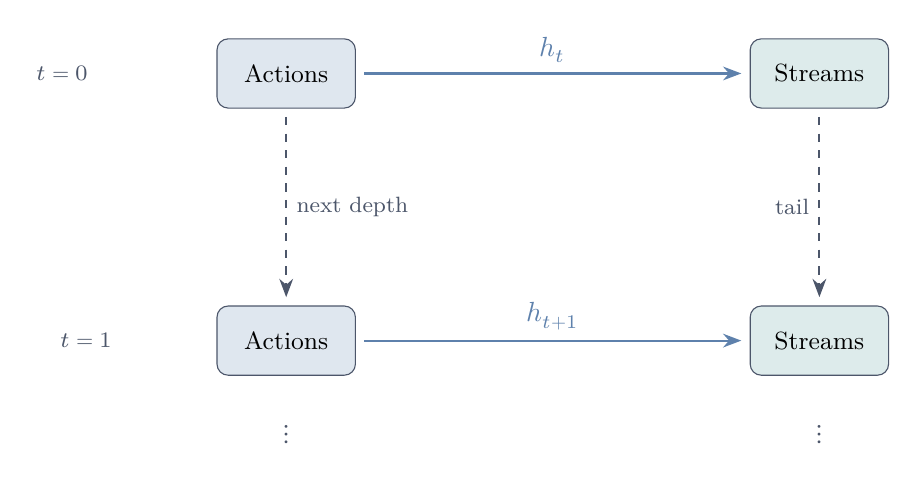
\begin{tikzpicture}[
    node distance=2.5cm and 5cm,
    obj/.style={draw=nord3,rounded corners,minimum height=2.5em,minimum width=5em,align=center,font=\small,fill=nord5},
    arr/.style={->,thick,>=Stealth,shorten >=3pt,shorten <=3pt,nord10}
]
\node[obj,fill=nord9!25] (A1) {Actions};
\node[obj,fill=nord7!30,right=of A1] (S1) {Streams};
\draw[arr] (A1) -- node[above,color=nord10] {$h_t$} (S1);

\node[obj,fill=nord9!25,below=of A1] (A2) {Actions};
\node[obj,fill=nord7!30,right=of A2] (S2) {Streams};
\draw[arr] (A2) -- node[above,color=nord10] {$h_{t+1}$} (S2);

\draw[arr,dashed,nord3] (A1) -- node[right,font=\footnotesize,color=nord3] {next depth} (A2);
\draw[arr,dashed,nord3] (S1) -- node[left,font=\footnotesize,color=nord3] {tail} (S2);

\node[below=0.5cm of A2,color=nord3] {$\vdots$};
\node[below=0.5cm of S2,color=nord3] {$\vdots$};

\node[left=1.5cm of A1,font=\footnotesize,color=nord3] {$t=0$};
\node[left=1.2cm of A2,font=\footnotesize,color=nord3] {$t=1$};
\end{tikzpicture}
\caption{The coinductive tower: $h_t$ maps each action to its successor-value stream at depth~$t$.  Ranking preservation ($a \le_a b \Rightarrow h_t(a) \le_s h_t(b)$) must hold at every level, verified by unfolding one \texttt{tail} at a time.}
\label{fig:tower}
\end{figure}

This is a \textbf{strategic} evaluation of actions: it assesses the absolute potential of the successor state, allowing for immediate tactical sacrifices.

\subsection{The Action-Value Specialization}

The coinductive homomorphism evaluates successor state quality---the agent's future \emph{after} the transition.  A natural strengthening evaluates the \emph{entire} consequence of an action, including the immediate reward it produces.

Given action~$a$ at state~$s$, define the \emph{action-value stream}:
\[
\mathit{action\text{-}value}(s,a) = \bigl[\, r(s,a),\;\; v_0,\;\; v_1,\;\; v_2,\;\; \ldots \,\bigr]
\]
Its head is the immediate transition reward; its tail is the value stream of the successor state.  The action-value stream is a richer object: it records both what the action pays now and what it sets up for the future.

\begin{definition}[Action-Value Coinductive Homomorphism]\label{def:coindhomo}
The ranking $\le_a$ is an \textbf{action-value coinductive homomorphism} at state~$s$ if:
\[
a \le_a b \;\;\Longrightarrow\;\; \mathit{action\text{-}value}(s,a) \le_s \mathit{action\text{-}value}(s,b)
\]
\end{definition}

\noindent Because $\le_s$ compares streams pointwise, this bundles \emph{two} requirements into one: the immediate rewards must compare correctly (the head), \emph{and} the successor state qualities must compare correctly (the tail).

This is a \textbf{tactical} evaluation: it demands that the better-ranked action wins both the immediate payoff and the long-term future.  When both conditions hold, the ranking is unassailable.  But when the optimal action sacrifices immediate reward for a superior successor---the pattern from Section~\ref{sec:key-idea}---the head condition breaks, and this definition cannot express the correct ranking.

\subsection{Decomposition}

The relationship between the two definitions is precise:

\begin{theorem}[Decomposition]\label{thm:decomposition}
The action-value condition decomposes into two independent conditions:
\begin{enumerate}
\item \textbf{Successor quality} (CoinductiveHomomorphism): $a \le_a b \implies \mathit{value}(\mathit{next}(s,a)) \le_s \mathit{value}(\mathit{next}(s,b))$
\item \textbf{Immediate reward compatibility}: $a \le_a b \implies r(s,a) \le_r r(s,b)$
\end{enumerate}
Either condition can hold independently.  Together, they are equivalent to the action-value condition.
\end{theorem}

The first condition is the coinductive homomorphism---the strategic evaluation.
The second is a purely local constraint on immediate rewards.
The action-value condition is their conjunction: it insists on tactical \emph{and} strategic soundness simultaneously.

When immediate rewards are aligned with the ranking---as they are in environments with uniform step costs, shaped rewards, or goal-terminal structure---the second condition holds for free, and the two definitions coincide.  The gap opens only in environments where the optimal action has a worse immediate reward than a suboptimal alternative: the sacrifice pattern.

\begin{figure}[H]
\centering
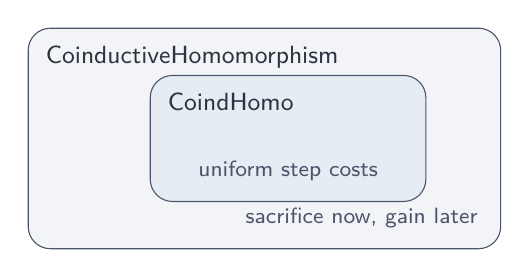
\begin{tikzpicture}[
    set/.style={draw=nord3,rounded corners=8pt,minimum width=6cm,minimum height=2.8cm,fill=nord5!50},
    label/.style={font=\small\sffamily,color=nord0},
    example/.style={font=\footnotesize\sffamily,color=nord3}
]
\node[set] (outer) {};
\node[set,minimum width=3.5cm,minimum height=1.6cm,fill=nord9!20,xshift=0.3cm] (inner) {};
\node[label,anchor=north west] at ([shift={(3pt,-3pt)}]outer.north west) {CoinductiveHomomorphism};
\node[label,anchor=north west] at ([shift={(3pt,-3pt)}]inner.north west) {CoindHomo};
\node[example,anchor=south] at ([yshift=4pt]inner.south) {uniform step costs};
\node[example,anchor=south east] at ([shift={(-5pt,4pt)}]outer.south east) {sacrifice now, gain later};
\end{tikzpicture}
\caption{CoindHomo is strictly contained in CoinductiveHomomorphism.  Environments with uniform step costs satisfy both.  Environments requiring immediate reward sacrifice separate them.}
\label{fig:containment}
\end{figure}

%%%%%%%%%%%%%%%%%%%%%%%%%%%%%%%%%%%%%%%%%%%%%%%%%%%%%%%%%%%%%%%%%%%%%%%%%%%%%%%
% PART IV: THE AGDA CORE
%%%%%%%%%%%%%%%%%%%%%%%%%%%%%%%%%%%%%%%%%%%%%%%%%%%%%%%%%%%%%%%%%%%%%%%%%%%%%%%

\section{The Agda Core}\label{sec:agda-core}

We now present the verified implementation.  This code is \emph{literate}---compiling this file with \texttt{agda --latex} type-checks everything while producing this PDF.

\begin{code}
{-# OPTIONS --safe --guardedness #-}

module CSHRL-Successor where

open import Data.List using (List; map; foldr; []; _∷_)
open import Codata.Guarded.Stream using (Stream; head; tail; _∷_; tabulate)
open import Relation.Binary.PropositionalEquality using (_≡_; _≢_; refl)
open import Data.Product using (proj₁; proj₂; _×_; _,_)
open import Relation.Nullary using (¬_; Dec; yes; no)
open import Function using (_∘_)
open import Data.Nat using (ℕ; zero; suc; _⊔_)
open import Data.Bool using (Bool; true; false; if_then_else_)
\end{code}

The \texttt{Core} module is parameterized by the environment:

\begin{code}
module Core
  (State Action Reward : Set)
  (step                : State → Action → State × Reward)
  (_≤ᵣ_                : Reward → Reward → Set)
  (max                 : Reward → Reward → Reward)
  (bottom              : Reward)
  (all-actions         : List Action)
  where

  infix 4 _≤ₛ_

  StreamR : Set
  StreamR = Stream Reward

  max-list : List Reward → Reward
  max-list = foldr max bottom
\end{code}

\subsection{Value and Action-Value Streams}

The key construction: \texttt{value} is an infinite stream obtained by tabulating finite-horizon solutions.

\begin{code}
  solve : State → ℕ → Reward
  solve s zero    = max-list (map (λ a → proj₂ (step s a)) all-actions)
  solve s (suc n) = max-list (map (λ a → solve (proj₁ (step s a)) n) all-actions)

  value : State → StreamR
  value s = tabulate (solve s)

  action-value : State → Action → StreamR
  head (action-value s a) = proj₂ (step s a)
  tail (action-value s a) = value (proj₁ (step s a))
\end{code}

\noindent \texttt{solve~s~n} computes the maximum reward achievable \emph{exactly~$n$ steps from now}, independently maximizing the action at every intermediate step.  Crucially, the action sequence that maximizes the reward at depth~$n$ may differ from the one that maximizes at depth~$m$.  The resulting value stream is therefore \emph{not a trajectory}---no single action sequence produces it.  It is the pointwise upper envelope of all possible trajectories: the agent's \textbf{capability profile} from state~$s$, recording the best it \emph{could} achieve at each future depth.

CoinductiveHomomorphism compares these capability profiles.  When state~$s_b$'s profile dominates~$s_a$'s at every depth, the agent prefers any action that reaches~$s_b$---even if that action sacrifices immediate reward.  The sacrifice is invisible in the profile: it only records what the agent \emph{can} reach, not the cost of getting there.

The \texttt{action-value} of action~$a$ at state~$s$ is a stream whose head is the immediate reward and whose tail is the capability profile of the successor state.

\subsection{Coinductive Stream Ordering}

\begin{code}
  record _≤ₛ_ (x y : StreamR) : Set where
    coinductive
    field
      head≤ : head x ≤ᵣ head y
      tail≤ : tail x ≤ₛ tail y

  open _≤ₛ_ public
\end{code}

\noindent A proof of $x \le_s y$ is an infinite witness: at every time step, the heads compare correctly.

\subsection{Why Propositions Instead of Booleans?}\label{sec:props-vs-bools}

The reward ordering \texttt{\_$\le$ᵣ\_} lives in \texttt{Set}---it is a \emph{proposition}, not a Boolean decision procedure.  This is a deliberate design choice:

\begin{itemize}
\item \textbf{Booleans are blind:} \texttt{true} carries no information about \emph{why} the comparison holds.  To use a Boolean result in a proof, a separate soundness lemma is required.
\item \textbf{Propositions carry evidence:} A value of type \texttt{r₁ $\le$ᵣ r₂} \emph{is} the proof---no lemma needed.
\item \textbf{Decidability bridges both:} \texttt{Dec (r₁ $\le$ᵣ r₂)} is either \texttt{yes p} (with proof~\texttt{p}) or \texttt{no ¬p} (with refutation).
\end{itemize}

\noindent This separation threads through the entire architecture: the Core module uses propositions for proofs; the Finder uses Booleans for speed; the Environment Class infrastructure bridges them via \texttt{Dec}.

\subsection{CoindHomo: The Action-Value Condition}

The \texttt{CoindHomo} record is the Agda encoding of the Action-Value Coinductive Homomorphism (Definition~\ref{def:coindhomo}):

\begin{code}
  record CoindHomo : Set₁ where
    field
      _≤ₐ_      : State → Action → Action → Set
      preserves : ∀ a b s → _≤ₐ_ s a b →
                  action-value s a ≤ₛ action-value s b

  open CoindHomo {{...}} public
\end{code}

\noindent The record has two fields.  The first, \texttt{\_$\le$ₐ\_}, is the ranking itself---a ternary relation indexed by state, taking two actions and returning a type (a proposition, per \S\ref{sec:props-vs-bools}).  The second, \texttt{preserves}, is the proof obligation: for any actions~$a, b$ and state~$s$, if the ranking says $a \le_a b$, then the full action-value stream of~$a$ is coinductively dominated by that of~$b$.  Because $\le_s$ checks both head and tail, this bundles two requirements: the immediate reward must compare correctly (head), and the successor state quality must compare correctly (tail).

\subsection{CoinductiveHomomorphism: The Successor Condition}

The \texttt{CoinductiveHomomorphism} record is the Agda encoding of Definition~\ref{def:coind-homo}.  The successor map extracts the state reached by an action:

\begin{code}
  next : State → Action → State
  next s a = proj₁ (step s a)

  successor-value : State → Action → StreamR
  successor-value s a = value (next s a)
\end{code}

\noindent \texttt{successor-value}~$s$~$a$ is the optimal value stream from the state reached by taking action~$a$ at state~$s$.  It is definitionally equal to $\mathit{tail}(\mathit{action\text{-}value}\;s\;a)$.

\begin{code}
  record CoinductiveHomomorphism : Set₁ where
    field
      _≤ₐ_      : State → Action → Action → Set
      preserves : ∀ a b s → _≤ₐ_ s a b →
                  successor-value s a ≤ₛ successor-value s b
\end{code}

\noindent CoinductiveHomomorphism requires only that the ranking preserves successor state quality.  The immediate transition reward is decoupled by design.

\subsection{The Decomposition}

\begin{code}
  CoindHomo→CoinductiveHomomorphism : CoindHomo → CoinductiveHomomorphism
  CoindHomo→CoinductiveHomomorphism homo = record
    { _≤ₐ_ = CoindHomo._≤ₐ_ homo
    ; preserves = λ a b s prf → tail≤ (CoindHomo.preserves homo a b s prf)
    }
\end{code}

\noindent Every CoindHomo is a CoinductiveHomomorphism: project the tail of the action-value stream dominance.  The converse does \emph{not} hold.

\begin{code}[hide]
  private
    combine-≤ₛ : ∀ {s a b} →
      proj₂ (step s a) ≤ᵣ proj₂ (step s b) →
      successor-value s a ≤ₛ successor-value s b →
      action-value s a ≤ₛ action-value s b
    head≤ (combine-≤ₛ h _) = h
    tail≤ (combine-≤ₛ _ t) = t
\end{code}

\begin{code}
  CoinductiveHomomorphism+Head→CoindHomo :
    (ch : CoinductiveHomomorphism) →
    (∀ a b s → CoinductiveHomomorphism._≤ₐ_ ch s a b →
      proj₂ (step s a) ≤ᵣ proj₂ (step s b)) →
    CoindHomo
  CoinductiveHomomorphism+Head→CoindHomo ch head-compat = record
    { _≤ₐ_ = CoinductiveHomomorphism._≤ₐ_ ch
    ; preserves = λ a b s prf →
        combine-≤ₛ (head-compat a b s prf)
                   (CoinductiveHomomorphism.preserves ch a b s prf)
    }
\end{code}

\noindent When immediate transition rewards also respect the ranking, CoinductiveHomomorphism specializes to CoindHomo.  This characterizes exactly what CoindHomo adds: the head constraint, which is orthogonal to successor state quality.

%%%%%%%%%%%%%%%%%%%%%%%%%%%%%%%%%%%%%%%%%%%%%%%%%%%%%%%%%%%%%%%%%%%%%%%%%%%%%%%
% PART V: THE LANDSCAPE
%%%%%%%%%%%%%%%%%%%%%%%%%%%%%%%%%%%%%%%%%%%%%%%%%%%%%%%%%%%%%%%%%%%%%%%%%%%%%%%

\section{When the Conditions Coincide---and When They Diverge}\label{sec:landscape}

The decomposition theorem reveals that CoindHomo and CoinductiveHomomorphism differ by exactly one condition: whether immediate transition rewards respect the ranking.  When does this matter?

\subsection{Aligned Environments: The Common Case}

In a large class of environments, the head condition holds trivially---and the two definitions coincide.  This class includes:

\begin{itemize}
\item \textbf{Uniform step costs.}  If all actions at a given state yield the same immediate reward, the head condition reduces to $r \le_r r$---reflexivity.  Examples: FrozenLake (all non-terminal steps give~$0$), MountainCar (all steps give~$-1$), navigation grids with uniform penalties.

\item \textbf{Shaped rewards.}  When reward functions are engineered so that immediate feedback points toward the optimal policy, the head condition is satisfied by construction.  This is common in continuous-control benchmarks (Pendulum, LunarLander) where shaping rewards guide the agent toward desirable configurations.

\item \textbf{Goal-terminal environments.}  If the episode ends upon reaching a goal state and all non-terminal transitions have equal cost, the only reward distinction is reaching the goal versus not.  The head condition holds at every non-terminal state.
\end{itemize}

For these environments, every CoinductiveHomomorphism is automatically a CoindHomo, and vice versa.  Results proved under CoindHomo---the Finder algorithm, propagation theorems, environment class constructions, verified instantiations---apply directly and without modification.  The environments are not ``easier'' in any pejorative sense; they are the standard decision problems that the reinforcement learning community has studied for decades, and they are well-served by either condition.

\subsection{The Sacrifice Pattern: An Unexplored Realm}

The gap between the two conditions opens when the optimal action has a \emph{worse} immediate reward than a suboptimal alternative.  We call this the \textbf{sacrifice pattern}: the agent must pay an immediate cost to reach a superior successor state.

This pattern is structurally interesting because it is precisely where discount factors also struggle.  A discount factor~$\gamma < 1$ exponentially suppresses future rewards; a sacrifice whose payoff arrives $k$~steps later is scaled by~$\gamma^k$.  For deep sacrifices---multi-stage investment chains, extended preparation sequences---the discounted return of the sacrificing action can fall below the myopic alternative, even though the undiscounted future is strictly superior at every depth.

CoindHomo and discounted returns thus share a blind spot: both anchor optimality to the present.  Discounting does so by geometric decay; CoindHomo does so via the head condition.  CoinductiveHomomorphism is the first condition in this framework that fully decouples optimality from immediate reward, judging actions solely by the quality of states they lead to.

\subsection{Why the Sacrifice Pattern Is Rare in Benchmarks}

The observation that CoindHomo suffices for virtually every standard environment is not a coincidence.  Reinforcement learning benchmarks have been developed in a culture where discounted scalar return is the optimality criterion.  Reward functions are carefully shaped to \emph{eliminate} the sacrifice pattern---that is literally the purpose of reward shaping.  Environments where immediate rewards actively mislead are regarded as ``hard exploration problems'' and are typically studied as pathological cases rather than representative ones.

The result is a selection bias: the environments that survive into textbooks and standard libraries are precisely those where immediate rewards already point toward optimality.  The sacrifice pattern---where the greedy action is wrong---has been quietly engineered out.

This does not diminish the value of CoindHomo.  It is the right tool for aligned environments, and the vast majority of practical decision problems have this structure.  Both conditions are introduced here as part of a unified framework: CoindHomo handles the common case cleanly, while CoinductiveHomomorphism extends the formal reach to environments where immediate rewards conflict with long-term quality---without losing anything that CoindHomo provides.

%%%%%%%%%%%%%%%%%%%%%%%%%%%%%%%%%%%%%%%%%%%%%%%%%%%%%%%%%%%%%%%%%%%%%%%%%%%%%%%
% PART VI: STRICT GENERALITY
%%%%%%%%%%%%%%%%%%%%%%%%%%%%%%%%%%%%%%%%%%%%%%%%%%%%%%%%%%%%%%%%%%%%%%%%%%%%%%%

\section{Strict Generality: Verified Counterexamples}\label{sec:strict-generality}

The implication CoindHomo $\Rightarrow$ CoinductiveHomomorphism is strict.  We prove this with three verified environments of increasing structural complexity, each exhibiting the sacrifice pattern.

\subsection{Sacrifice Now, Gain Later}

The minimal separating example has three states and two actions:

\begin{center}
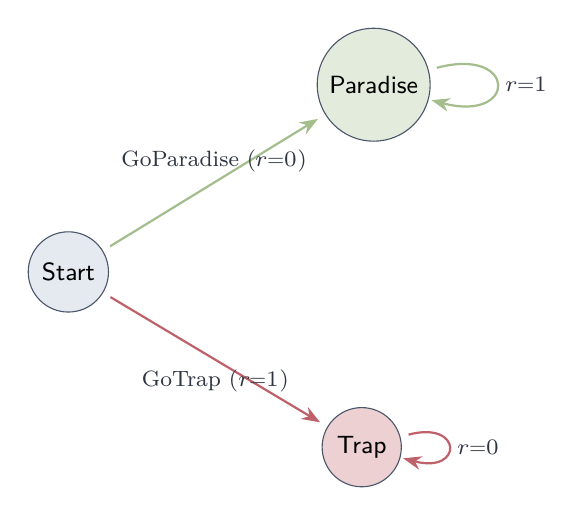
\begin{tikzpicture}[
    state/.style={draw=nord3,circle,minimum size=2em,font=\small\sffamily,fill=nord5},
    arr/.style={->,thick,>=Stealth,shorten >=3pt,shorten <=3pt}
]
\node[state] (S) {Start};
\node[state,above right=1.5cm and 3cm of S,fill=nord14!30] (P) {Paradise};
\node[state,below right=1.5cm and 3cm of S,fill=nord11!30] (T) {Trap};

\draw[arr,nord14] (S) -- node[above,font=\footnotesize,color=nord0] {GoParadise ($r{=}0$)} (P);
\draw[arr,nord11] (S) -- node[below,font=\footnotesize,color=nord0] {GoTrap ($r{=}1$)} (T);
\draw[arr,nord14] (P) edge[loop right] node[right,font=\footnotesize,color=nord0] {$r{=}1$} (P);
\draw[arr,nord11] (T) edge[loop right] node[right,font=\footnotesize,color=nord0] {$r{=}0$} (T);
\end{tikzpicture}
\end{center}

GoParadise sacrifices the immediate reward ($0$ vs~$1$) but leads to Paradise (reward~$1$ forever).  GoTrap grabs the immediate reward but leads to Trap (reward~$0$ forever).

\textbf{CoinductiveHomomorphism:} $\mathit{value}(\text{Trap}) = [0,0,\ldots] \le_s [1,1,\ldots] = \mathit{value}(\text{Paradise})$ \checkmark

\textbf{CoindHomo:} Cannot rank GoTrap $\le$ GoParadise (head requires $1 \le 0$). Cannot rank GoParadise $\le$ GoTrap either (tail comparison yields $1 \le 0$ at the head of the successor streams). The actions are \emph{incomparable}---even though one is clearly better.

Full proof: \fpath{src/CSHRL/Tasks/Verified/BinarySacrifice.agda}

\subsection{Skill Investment: Multi-Stage Sacrifice}

A chain of investment decisions where training sacrifices immediate reward to advance:

\begin{center}
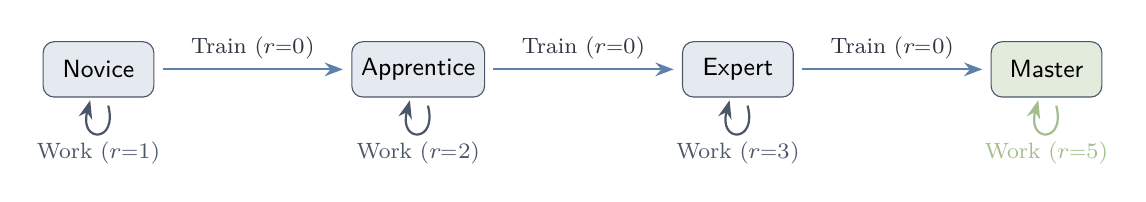
\begin{tikzpicture}[
    state/.style={draw=nord3,rounded corners,minimum size=2em,font=\small\sffamily,fill=nord5,minimum width=4em},
    arr/.style={->,thick,>=Stealth,shorten >=3pt,shorten <=3pt}
]
\node[state] (N) {Novice};
\node[state,right=2.5cm of N] (A) {Apprentice};
\node[state,right=2.5cm of A] (E) {Expert};
\node[state,right=2.5cm of E,fill=nord14!30] (M) {Master};

\draw[arr,nord10] (N) -- node[above,font=\footnotesize,color=nord0] {Train ($r{=}0$)} (A);
\draw[arr,nord10] (A) -- node[above,font=\footnotesize,color=nord0] {Train ($r{=}0$)} (E);
\draw[arr,nord10] (E) -- node[above,font=\footnotesize,color=nord0] {Train ($r{=}0$)} (M);

\draw[arr,nord3] (N) edge[loop below] node[below,font=\footnotesize,color=nord3] {Work ($r{=}1$)} (N);
\draw[arr,nord3] (A) edge[loop below] node[below,font=\footnotesize,color=nord3] {Work ($r{=}2$)} (A);
\draw[arr,nord3] (E) edge[loop below] node[below,font=\footnotesize,color=nord3] {Work ($r{=}3$)} (E);
\draw[arr,nord14] (M) edge[loop below] node[below,font=\footnotesize,color=nord14] {Work ($r{=}5$)} (M);
\end{tikzpicture}
\end{center}

The capability profiles (value streams) form a clean progression:
\[
\begin{aligned}
\text{Master:}\quad     &[5, 5, 5, 5, \ldots] \\
\text{Expert:}\quad     &[3, 5, 5, 5, \ldots] \\
\text{Apprentice:}\quad &[2, 3, 5, 5, \ldots] \\
\text{Novice:}\quad     &[1, 2, 3, 5, \ldots]
\end{aligned}
\]

\noindent These are \emph{not trajectories}.  Consider the Apprentice profile~$[2, 3, 5, \ldots]$: the~$2$ at depth~$0$ comes from Working (best immediate reward), the~$3$ at depth~$1$ comes from Training to Expert \emph{then} Working (a different action plan), and the~$5$ at depth~$2$ comes from Training twice to Master then Working (yet another plan).  Each entry independently records the best the agent \emph{could} achieve at that depth.  No single action sequence produces the stream $[2, 3, 5, \ldots]$.

CoinductiveHomomorphism compares these profiles: Train's successor (Expert, profile~$[3,5,5,\ldots]$) pointwise dominates Work's successor (Apprentice, profile~$[2,3,5,\ldots]$).  The sacrifice---Train's immediate reward of~$0$ versus Work's~$2$---does not appear in the successor profiles, because the profiles record reachable capability, not incurred cost.

CoindHomo fails at every level: Work's immediate reward always exceeds Train's, so the action-value streams are pointwise incomparable.

Full proof: \fpath{src/CSHRL/Tasks/Verified/SkillInvestment.agda}

\subsection{Preparation Dilemma: Cyclic Dynamics}

A structurally different pattern with regression and context-dependent optimal actions:

\begin{center}
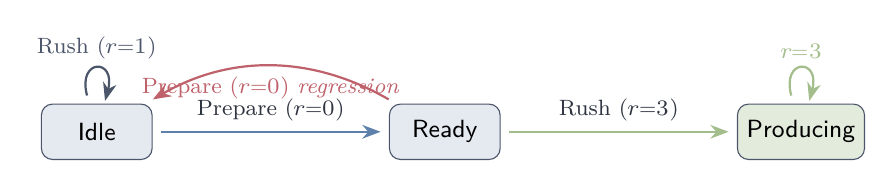
\begin{tikzpicture}[
    state/.style={draw=nord3,rounded corners,minimum size=2em,font=\small\sffamily,fill=nord5,minimum width=4em},
    arr/.style={->,thick,>=Stealth,shorten >=3pt,shorten <=3pt}
]
\node[state] (I) {Idle};
\node[state,right=3cm of I] (R) {Ready};
\node[state,right=3cm of R,fill=nord14!30] (P) {Producing};

\draw[arr,nord10] (I) -- node[above,font=\footnotesize,color=nord0] {Prepare ($r{=}0$)} (R);
\draw[arr,nord14] (R) -- node[above,font=\footnotesize,color=nord0] {Rush ($r{=}3$)} (P);

\draw[arr,nord3] (I) edge[loop above] node[above,font=\footnotesize,color=nord3] {Rush ($r{=}1$)} (I);
\draw[arr,nord11] (R) edge[bend right=30] node[below,font=\footnotesize,color=nord11] {Prepare ($r{=}0$) \emph{regression}} (I);
\draw[arr,nord14] (P) edge[loop above] node[above,font=\footnotesize,color=nord14] {$r{=}3$} (P);
\end{tikzpicture}
\end{center}

\noindent At Idle, the optimal action is Prepare (sacrifice now for readiness).  At Ready, the optimal action flips to Rush (capitalize on preparation).  Over-preparing at Ready sends the agent \emph{back} to Idle---a regression penalty.

Value streams: $\text{Producing} = \text{Ready} = [3,3,3,\ldots]$, $\text{Idle} = [1,3,3,\ldots]$.

CoinductiveHomomorphism handles the context-dependent ranking: Prepare $>$ Rush at Idle (successor quality improves), Rush $>$ Prepare at Ready (successor quality improves).

CoindHomo cannot rank the actions at Idle in \emph{either} direction:
\begin{itemize}
\item Forward (Rush $\le$ Prepare): head requires $1 \le 0$---absurd.
\item Reverse (Prepare $\le$ Rush): head is $0 \le 1$ (ok), but the tail requires $\mathit{value}(\text{Ready}) \le_s \mathit{value}(\text{Idle})$, which fails at the head: $3 \le 1$---absurd.
\end{itemize}

Full proof: \fpath{src/CSHRL/Tasks/Verified/PreparationDilemma.agda}

%%%%%%%%%%%%%%%%%%%%%%%%%%%%%%%%%%%%%%%%%%%%%%%%%%%%%%%%%%%%%%%%%%%%%%%%%%%%%%%
% PART VII: SUBSUMPTION
%%%%%%%%%%%%%%%%%%%%%%%%%%%%%%%%%%%%%%%%%%%%%%%%%%%%%%%%%%%%%%%%%%%%%%%%%%%%%%%

\section{Subsumption and Classical RL}\label{sec:subsumes}

The value streams compared by CoinductiveHomomorphism are computed from the actual environment dynamics by the \texttt{solve} function---they are ground truth, not estimates.  If the environment terminates (absorbing states with zero reward), the value streams reflect that.  If the environment is infinite, the streams extend accordingly.  The horizon is not a parameter of the condition; it is encoded in the dynamics.

\subsection{CoindHomo Subsumes Discounted Return}

The action-value condition compares the \emph{full} action-value streams, which include the immediate reward as the head element.  Pointwise dominance at every position implies that the cumulative sum---at every finite horizon---is at least as large for the better-ranked action.  Since the discounted return is a weighted sum with positive weights, action-value dominance implies discounted return dominance for every discount factor $\gamma \in [0,1)$.

This is genuine subsumption: any policy optimal under CoindHomo is also optimal under every discounted return criterion.

\subsection{CoinductiveHomomorphism Subsumes Successor Return}

The coinductive homomorphism compares successor value streams---the accumulated reward \emph{from the state the action leads to}.  The verified theorem states:

\begin{code}[hide]
  iter-head : ℕ → StreamR → Reward
  iter-head zero    s = head s
  iter-head (suc n) s = iter-head n (tail s)

  PointwiseDominance : StreamR → StreamR → Set
  PointwiseDominance x y = ∀ n → iter-head n x ≤ᵣ iter-head n y

  ≤ₛ-to-pointwise : ∀ {x y} → x ≤ₛ y → PointwiseDominance x y
  ≤ₛ-to-pointwise p zero    = head≤ p
  ≤ₛ-to-pointwise p (suc n) = ≤ₛ-to-pointwise (tail≤ p) n
\end{code}

\begin{code}[hide]
module CoreWithArithmetic
  (State Action Reward : Set)
  (step                : State → Action → State × Reward)
  (_≤ᵣ_                : Reward → Reward → Set)
  (max                 : Reward → Reward → Reward)
  (bottom              : Reward)
  (all-actions         : List Action)
  (_+ᵣ_                : Reward → Reward → Reward)
  (≤ᵣ-refl             : ∀ {r} → r ≤ᵣ r)
  (+ᵣ-mono-≤           : ∀ {a b c d} → a ≤ᵣ b → c ≤ᵣ d → (a +ᵣ c) ≤ᵣ (b +ᵣ d))
  where

  open Core State Action Reward step _≤ᵣ_ max bottom all-actions public

  pointwise-tail : ∀ {x y} → PointwiseDominance x y → PointwiseDominance (tail x) (tail y)
  pointwise-tail pw n = pw (suc n)

  partial-sum : ℕ → StreamR → Reward
  partial-sum zero    _ = bottom
  partial-sum (suc n) s = head s +ᵣ partial-sum n (tail s)

  partial-sum-mono : ∀ N x y → PointwiseDominance x y →
                     partial-sum N x ≤ᵣ partial-sum N y
  partial-sum-mono zero _ _ _ = ≤ᵣ-refl
  partial-sum-mono (suc n) x y pw =
    +ᵣ-mono-≤ (pw zero) (partial-sum-mono n (tail x) (tail y) (pointwise-tail pw))
\end{code}

\begin{code}
  subsumes-successor-return : (ch : CoinductiveHomomorphism) →
    ∀ s a b N →
    CoinductiveHomomorphism._≤ₐ_ ch s a b →
    partial-sum N (successor-value s a) ≤ᵣ
    partial-sum N (successor-value s b)
  subsumes-successor-return ch s a b N p =
    partial-sum-mono N _ _ (≤ₛ-to-pointwise
      (CoinductiveHomomorphism.preserves ch a b s p))
\end{code}

\noindent The top-ranked action leads to the state with the highest accumulated reward at every finite horizon.  This is successor return dominance: the better-ranked action places the agent in a strictly better position.

\subsection{Where Discounted Return Fails}

To make the contrast with classical RL concrete, we examine Q-learning---the workhorse algorithm of model-free reinforcement learning~\cite{Sutton2018}.  Q-learning maintains a table of \emph{Q-values}, $Q(s, a)$, estimating the expected discounted return of taking action~$a$ in state~$s$ and acting optimally thereafter.  These estimates are updated via the Bellman equation:
\[
Q(s, a) \;\leftarrow\; r(s, a) \;+\; \gamma \cdot \max_{a'} Q(s', a')
\]
where $r(s,a)$ is the immediate reward, $s'$ is the successor state, and $\gamma \in [0, 1)$ is the discount factor.  The agent then selects the action with the highest Q-value: $\pi(s) = \arg\max_a Q(s, a)$.  Under standard conditions, Q-learning converges to the optimal Q-values, and the greedy policy is optimal \emph{for the discounted objective}.  The problem, as we now show, is that the discounted objective itself can be wrong.

In sacrifice environments, Q-learning can converge to a suboptimal policy---not because the algorithm fails, but because the discount factor distorts the objective it optimizes.  We demonstrate this concretely on the binary sacrifice MDP.

\paragraph{The verified ground truth.}
The \texttt{solve} function computes the optimal reward at each depth from the actual environment dynamics:
\[
\begin{aligned}
\text{solve}(\text{Paradise}, n) &= 1 \quad \text{for all } n \\
\text{solve}(\text{Trap}, n) &= 0 \quad \text{for all } n
\end{aligned}
\]
These are machine-verified facts, not estimates.  Paradise yields reward~$1$ at every future depth; Trap yields~$0$.  The accumulated reward from Paradise at horizon~$N$ is~$N$; from Trap it is~$0$.

\paragraph{The Q-value computation.}
The Bellman equation gives Q-learning's converged values at state Start:
\[
\begin{aligned}
Q(\text{Start}, \text{GoTrap})     &= \underbrace{1}_{\text{immediate}} + \gamma \cdot \underbrace{0}_{\textstyle V(\text{Trap})} = 1 \\[6pt]
Q(\text{Start}, \text{GoParadise}) &= \underbrace{0}_{\text{immediate}} + \gamma \cdot \underbrace{\tfrac{1}{1-\gamma}}_{\textstyle V(\text{Paradise})} = \tfrac{\gamma}{1-\gamma}
\end{aligned}
\]
For $\gamma < \tfrac{1}{2}$, we have $\tfrac{\gamma}{1-\gamma} < 1$, so Q-learning selects GoTrap---the action whose successor state has accumulated reward~$0$ at every horizon---over GoParadise, whose successor state has accumulated reward~$N$ at horizon~$N$.

The discount factor $\gamma$ geometrically suppresses $V(\text{Paradise})$, which is the only term that carries the evidence of Paradise's superiority.  When $\gamma$ is small enough, the suppression is sufficient to make a state worth $[1,1,1,\ldots]$ appear less valuable than a state worth $[0,0,0,\ldots]$.

\paragraph{The verified conclusion.}
We prove in Agda (\fpath{src/CSHRL/Analysis/QLearningFailure.agda}) the conjunction of two facts:
\begin{enumerate}
\item \textbf{Tactical:} $r(\text{Start}, \text{GoParadise}) \le r(\text{Start}, \text{GoTrap})$ --- GoTrap has the higher immediate reward.
\item \textbf{Strategic:} For every horizon~$N$, the accumulated reward from GoParadise's successor exceeds GoTrap's:
\[
\sum_{i=0}^{N-1} \text{solve}(\text{Trap}, i) \;\le\; \sum_{i=0}^{N-1} \text{solve}(\text{Paradise}, i)
\]
\end{enumerate}
Together: Q-learning with $\gamma < \tfrac{1}{2}$ selects the action with the higher immediate reward and the strictly inferior successor state.  The discount factor is the mechanism by which the tactical advantage overrides the strategic one.

\paragraph{Deeper sacrifice chains.}
The Skill Investment chain sharpens the point.  Q-learning requires $\gamma > (1/5)^{1/3} \approx 0.585$ to identify the optimal training path.  Below this threshold, it converges to the policy of working at Novice forever---earning~$1$ per step while a three-step investment would yield~$5$ per step permanently.  CoinductiveHomomorphism identifies the training path regardless: the successor state quality is strictly better at every depth, and the environment dynamics confirm it.

\subsection{CoindHomo as a Conservative Strengthening}

When the two conditions coincide---in environments where immediate rewards align with the ranking---CoinductiveHomomorphism inherits CoindHomo's full subsumption of classical RL.  This covers the vast majority of standard environments (Section~\ref{sec:landscape}).

In sacrifice environments, CoindHomo cannot rank the actions at all (the action-value streams are pointwise incomparable), while CoinductiveHomomorphism correctly identifies the better successor state.  CoindHomo is the conservative choice: it refuses to rank when the immediate reward conflicts with the future.  CoinductiveHomomorphism resolves the conflict in favor of successor state quality---which the environment dynamics validate.

%%%%%%%%%%%%%%%%%%%%%%%%%%%%%%%%%%%%%%%%%%%%%%%%%%%%%%%%%%%%%%%%%%%%%%%%%%%%%%%
% PART VIII: STREAM ISOMORPHISM
%%%%%%%%%%%%%%%%%%%%%%%%%%%%%%%%%%%%%%%%%%%%%%%%%%%%%%%%%%%%%%%%%%%%%%%%%%%%%%%

\section{The Stream Isomorphism}\label{sec:stream-iso}

We defined stream dominance coinductively: $x \le_s y$ iff heads compare and tails recursively compare.  A natural question is whether this definition captures exactly pointwise dominance at every timestep.  The answer is affirmative: the coinductive definition is \emph{isomorphic} to pointwise dominance.

The forward direction (\texttt{≤ₛ-to-pointwise}) was already given in \S\ref{sec:agda-core}.  The reverse:

\begin{code}[hide]
module IsoSketch
  (Reward : Set)
  (_≤ᵣ_ : Reward → Reward → Set)
  where
  
  open import Data.Nat using (ℕ; zero; suc)
  
  record StreamR : Set where
    coinductive
    field head : Reward
          tail : StreamR
  open StreamR public
  
  iter-head : ℕ → StreamR → Reward
  iter-head zero s = head s
  iter-head (suc n) s = iter-head n (tail s)
  
  PointwiseDominance : StreamR → StreamR → Set
  PointwiseDominance x y = ∀ n → iter-head n x ≤ᵣ iter-head n y

  record _≤ₛ_ (x y : StreamR) : Set where
    coinductive
    field head≤ : head x ≤ᵣ head y
          tail≤ : tail x ≤ₛ tail y
  open _≤ₛ_ public
  
  pointwise-tail : ∀ {x y} → PointwiseDominance x y → PointwiseDominance (tail x) (tail y)
  pointwise-tail pw n = pw (suc n)
\end{code}

\begin{code}
  pointwise-to-≤ₛ : ∀ {x y} → PointwiseDominance x y → x ≤ₛ y
  head≤ (pointwise-to-≤ₛ pw) = pw zero
  tail≤ (pointwise-to-≤ₛ pw) = pointwise-to-≤ₛ (pointwise-tail pw)
\end{code}

\noindent Together with \texttt{≤ₛ-to-pointwise}, this yields:
\[
x \le_s y \;\Longleftrightarrow\; \forall n.\, x_n \le_r y_n
\]

This isomorphism has three consequences.  First, it confirms that the coinductive formulation exactly captures ``dominance at every timestep''---it is a precise characterization, not an approximation.  Second, it establishes Finder completeness: since the Finder compares traces at finite depths, the isomorphism guarantees that trace dominance at all depths implies coinductive stream dominance.  Third, the bidirectional correspondence means that rankings preserving stream order and stream orders inducing rankings are interchangeable views---the ``symmetric'' aspect of the framework.

The isomorphism applies equally to both CoinductiveHomomorphism and CoindHomo: both use $\le_s$ as their codomain ordering, differing only in which streams are compared (successor value streams vs.\ action-value streams).

\noindent The full proof is in \fpath{src/appendix/StreamIsomorphism.agda}.

%%%%%%%%%%%%%%%%%%%%%%%%%%%%%%%%%%%%%%%%%%%%%%%%%%%%%%%%%%%%%%%%%%%%%%%%%%%%%%%
% PART VIII: THE ALGORITHM
%%%%%%%%%%%%%%%%%%%%%%%%%%%%%%%%%%%%%%%%%%%%%%%%%%%%%%%%%%%%%%%%%%%%%%%%%%%%%%%

\section{The Finder Algorithm}\label{sec:finder}

The preceding sections established what an optimal ranking \emph{is}.  We now turn to how to \emph{compute} one.  The Finder algorithm uses lexicographic trace comparison and requires no discount factor.

\begin{code}
module Finder
  (State Action Reward : Set)
  (step                : State → Action → State × Reward)
  (_≤?_                : Reward → Reward → Bool)
  (default-action      : Action)
  (all-actions         : List Action)
  where

  open import Data.List using (List; map)

  Trace : Set
  Trace = List Reward
\end{code}

\subsection{Lexicographic Comparison}

Compare traces element-by-element---the first difference decides:

\begin{code}
  _≤ₜ_ : Trace → Trace → Bool
  []       ≤ₜ []       = true
  []       ≤ₜ (_ ∷ _)  = true
  (_ ∷ _)  ≤ₜ []       = false
  (r₁ ∷ t₁) ≤ₜ (r₂ ∷ t₂) =
    if r₁ ≤? r₂ then
      if r₂ ≤? r₁ then (t₁ ≤ₜ t₂)
      else true
    else false
\end{code}

\noindent Unlike summation (which discards timing information), lexicographic comparison preserves it: a trace $[10, -5]$ dominates $[0, 5]$ because $10 > 0$ at step~$0$, regardless of subsequent elements.

\subsection{Trace Evaluation}

Given the comparator, we need the traces themselves.  For a deterministic MDP, the trace of action~$a$ at state~$s$ to depth~$k$ is the finite prefix of the reward stream: take action~$a$, record the reward, then act optimally (according to all actions, greedily at each step) for the remaining~$k{-}1$ steps.  \texttt{best-trace} computes this optimal continuation; \texttt{trace-action} prepends the immediate reward of a specific action:

\begin{code}
  mutual
    best-trace : State → ℕ → Trace
    best-trace s zero    = []
    best-trace s (suc k) =
      let outcomes = map (λ a → trace-action s a k) all-actions
      in max-trace outcomes

    trace-action : State → Action → ℕ → Trace
    trace-action s a k =
      let (s' , r) = step s a
          future   = best-trace s' k
      in r ∷ future

    max-trace : List Trace → Trace
    max-trace []       = []
    max-trace (t ∷ ts) = max-helper t ts

    max-helper : Trace → List Trace → Trace
    max-helper current [] = current
    max-helper current (t ∷ ts) =
      if current ≤ₜ t
      then max-helper t ts
      else max-helper current ts
\end{code}

\subsection{The Ranking Finder}

With traces and a comparator in hand, producing a ranking is straightforward: compute each action's trace at the desired depth, then sort by lexicographic dominance.  The head of the sorted list is the optimal action; the full list is the total ranking used by the adaptation layer (\S\ref{sec:adaptation}).

\begin{code}
  insert : (Action × Trace) → List (Action × Trace) → List (Action × Trace)
  insert x [] = x ∷ []
  insert (a₁ , t₁) ((a₂ , t₂) ∷ xs) =
    if t₂ ≤ₜ t₁
    then (a₁ , t₁) ∷ (a₂ , t₂) ∷ xs
    else (a₂ , t₂) ∷ insert (a₁ , t₁) xs

  sort-scored : List (Action × Trace) → List (Action × Trace)
  sort-scored [] = []
  sort-scored (x ∷ xs) = insert x (sort-scored xs)

  find-ranking : State → ℕ → List Action
  find-ranking s k =
    let scored = map (λ a → (a , trace-action s a k)) all-actions
        sorted = sort-scored scored
    in map proj₁ sorted

  find-policy : State → ℕ → Action
  find-policy s k =
    let ranking = find-ranking s k
    in head-default ranking
    where
      head-default : List Action → Action
      head-default []      = default-action
      head-default (x ∷ _) = x
\end{code}

\noindent No discount factor is required.  Standard RL needs $\gamma < 1$ to ensure convergence of the sum; here we compare structure directly, and the lexicographic order is well-defined at any depth.

\subsection{Serving Both Conditions}

The Finder as defined above computes \texttt{trace-action}---whose head is the immediate reward and whose tail is the optimal future.  This directly serves \textbf{CoindHomo}: action-value traces are the finite approximations of action-value streams.

For \textbf{CoinductiveHomomorphism}, the relevant comparison is between \emph{successor-value traces}---the optimal future from the state reached by each action, \emph{excluding} the immediate reward.  The adaptation is a one-line change: instead of \texttt{r~∷~future}, use \texttt{future} alone.  Equivalently, compare \texttt{tail(trace-action~s~a~k)} for each action.

In aligned environments (Section~\ref{sec:landscape}), both comparisons yield the same ranking.  In sacrifice environments, the action-value trace may be incomparable (the head reversal prevents lexicographic dominance), while the successor-value trace correctly identifies the better successor state.  The Stream Isomorphism (\S\ref{sec:stream-iso}) guarantees that trace dominance at all depths implies coinductive stream dominance---for whichever stream variant is used.

\section{Environment Classes: Modularity Without Postulates}\label{sec:env-classes}

The Finder produces rankings; the Stream Isomorphism connects them to coinductive stream dominance.  But each task still needs its own bridge lemma---a potentially tedious and error-prone process.  The \textbf{Environment Class} (EC) abstraction eliminates this boilerplate.  Rather than proving preservation from scratch for each task, we factor out common structure into reusable modules.

\subsection{The Problem: Boilerplate and Trust}

Without environment classes, every task would need:
\begin{enumerate}
\item Its own Finder algorithm implementation
\item Its own trace-to-stream bridge lemma
\item Its own preservation proof skeleton
\end{enumerate}

This leads to code duplication and, worse, \emph{trust issues}: which parts can be trusted vs.\ which need re-verification?

\subsection{The Solution: Parameterized Modules}

Environment classes provide \textbf{verified infrastructure} that task instances inherit.  A task author fills in a parameter record (types, step function, reward order), and the class automatically provides the Finder, trace types, stream bridges, and proof scaffolding.  The full implementation is in \fpath{src/CSHRL/EnvironmentClass/}; here we show the parameter record that a task must instantiate:

\begin{code}[hide]
module FiniteDeterministicMDPSignature where
  open import Data.Unit using (⊤)
  open import Data.Empty using (⊥)
\end{code}

\begin{code}
  record ECParameters : Set₁ where
    field
      State Action Reward : Set
      step      : State → Action → State × Reward
      _≤ᵣ_      : Reward → Reward → Set
      _≤?_      : (r s : Reward) → Dec (r ≤ᵣ s)
      ≤ᵣ-refl   : ∀ {r} → r ≤ᵣ r
      max       : Reward → Reward → Reward
      bottom    : Reward
      all-actions    : List Action
      default-action : Action
      horizon   : ℕ
\end{code}

\begin{code}[hide]
  module ECProvides (P : ECParameters) where
    open ECParameters P
    
    Trace : Set
    Trace = List Reward
    
    _≤ₜ_ : Trace → Trace → Set
    []       ≤ₜ []       = ⊤
    []       ≤ₜ (_ ∷ _)  = ⊤
    (_ ∷ _)  ≤ₜ []       = ⊥
    (r₁ ∷ t₁) ≤ₜ (r₂ ∷ t₂) = (r₁ ≤ᵣ r₂) × ((r₂ ≤ᵣ r₁) → t₁ ≤ₜ t₂)
\end{code}

\noindent The fields divide into three groups.  The \emph{domain} group (\texttt{State}, \texttt{Action}, \texttt{step}) specifies the MDP.  The \emph{algebraic} group (\texttt{\_$\le$ᵣ\_}, \texttt{\_$\le$?\_}, \texttt{max}, \texttt{bottom}) provides the ordered semiring structure on rewards, ensuring comparability and bounded extrema.  The \emph{enumeration} group (\texttt{all-actions}, \texttt{default-action}, \texttt{horizon}) supplies finiteness witnesses needed by the Finder's brute-force search.

Given these parameters, the environment class automatically provides:

\begin{code}
  -- AUTOMATICALLY PROVIDED by the EC:
  -- • Trace type and orderings (_≤ₜ_, _≤ₜᵇ_)
  -- • Finder algorithm (best-trace, find-ranking, find-policy)
  -- • Ranking relation (_ranks_≤_)
  -- • Trace-to-stream bridge infrastructure (trace-≤ₜ-head)
  -- • Stream reflexivity (≤ₛ-refl)
  -- • Full CoindHomo (for specialised ECs like CombinatorialPlacementMDP)
\end{code}

\subsection{What Task Instances Must Provide}\label{sec:task-provide}

The burden on a task instance depends on which environment class it instantiates.

\paragraph{FiniteDeterministicMDP (general case).}
A task provides:
\begin{enumerate}
\item \textbf{Domain specifics:} The \texttt{State}, \texttt{Action}, \texttt{step} function.
\item \textbf{A direct preservation proof:} A proof that the Finder's ranking preserves action-value ordering---the full bridge from finite traces to infinite streams.
\end{enumerate}

\paragraph{CombinatorialPlacementMDP (placement problems).}\label{sec:cpmdp}
A specialised EC for placement problems (N-Queens, Sudoku, Graph Coloring), extending FiniteDeterministicMDP with domain-specific structure.  The full implementation is in \fpath{src/CSHRL/EnvironmentClass/CombinatorialPlacementMDP.agda}:

\begin{code}[hide]
module CombinatorialPlacementSignature where
\end{code}

\begin{code}
  record PlacementParameters : Set₁ where
    field
      Config : Set
      Action : Set
      is-dead   : Config → Bool
      is-solved : Config → Bool
      place : Config → Action → Config
      solved-reward : ℕ
      all-actions : List Action
      default-action : Action
      horizon : ℕ

  data PlacementState (Config : Set) : Set where
    Ongoing : Config → PlacementState Config
    Dead    : PlacementState Config
    Solved  : Config → PlacementState Config
\end{code}

\noindent The three constructors model the life cycle of a placement problem: \texttt{Ongoing}~wraps an active configuration where pieces can still be placed; \texttt{Dead} is an absorbing failure state (e.g., two queens attacking each other with no remaining fix); \texttt{Solved} wraps a completed valid configuration.  The key structural property is that Dead states produce stream~$[0, 0, 0, \ldots]$ and Solved states produce~$[R, R, R, \ldots]$.  Any path reaching Solved therefore dominates any path reaching Dead at every timestep---precisely the condition required by the coinductive order.

The EC factors the preservation proof into reusable layers:

\begin{enumerate}
\item \texttt{WithAbsorbingLemmas} (parameters: \texttt{solve-Dead-0}, \texttt{solve-Solved-R}).  Derives stream-level domination lemmas for absorbing states.

\item \texttt{WithBinaryStructure} (adds: \texttt{0\textless{}R}).  Proves that \texttt{solve} is \emph{binary}---every value is either $0$ or $R$---and derives monotonicity.

\item \texttt{WithTraceBridge} (adds: \texttt{solve-horizon-suf}).  Combines binary structure with horizon sufficiency to construct the full \texttt{CoindHomo}: the Finder's trace-based ranking preserves the coinductive ordering of action-value streams.
\end{enumerate}

\noindent The task author supplies at most four simple ingredients (the placement parameters, two absorbing-state lemmas, and horizon sufficiency), while the EC machinery handles the entire bridge from finite traces to infinite streams.

\paragraph{Validation: 8-Queens ($N = 8$).}
The \texttt{Queens8} module (\fpath{src/CSHRL/Tasks/Verified/Queens8.agda}) instantiates the EC for the $8$-Queens problem with \texttt{--safe} and zero postulates.  With \texttt{solve-horizon-suf} discharged, opening \texttt{WithTraceBridge} yields a complete \texttt{CoindHomo}: for every state~$s$ and actions~$a, b$, if the Finder ranks $a \le b$, then the infinite reward stream of~$a$ is dominated by that of~$b$ at every time step.  This is achieved for a combinatorial search space ($8^8 = 16{,}777{,}216$ candidate placements) where direct stream enumeration is infeasible.

\subsection{Why This Matters: Postulate-Free Verification}

\begin{itemize}
\item \textbf{Verified tasks} (like TwoState, Queens1, and Queens8) have \textbf{no postulates}---every claim is machine-checked.
\item \textbf{Classic tasks} (like Maze, KeyDoor) can use postulates for properties that are difficult to formalise, but the \emph{structural} preservation proof is still verified.
\item \textbf{New tasks} inherit all the machinery---just instantiate the module parameters.
\end{itemize}

\begin{figure}[H]
\centering
\begin{tikzpicture}[
    node distance=0.8cm and 1.0cm,
    box/.style={draw,rounded corners,minimum height=2.0em,minimum width=5em,align=center,font=\footnotesize},
    groupbox/.style={draw,rounded corners,inner sep=0.3cm,fill=white},
    smallbox/.style={rounded corners,minimum height=1.4em,minimum width=3.5em,align=center,font=\tiny,fill=nord13!25},
    stochbox/.style={rounded corners,minimum height=1.4em,minimum width=3.5em,align=center,font=\tiny,fill=nord14!35},
    inherit/.style={->,thick,>=Stealth,dashed},
    arr/.style={->,>=Stealth}
]
\node[box,fill=nord9!20] (core) {Core.agda\\(Theory)};
\node[box,fill=nord15!20,right=3.5cm of core] (stoch) {Core/Stochastic\\(Giry monad)};

\node[box,fill=nord7!25,below left=1.0cm and 1.5cm of core] (fdmdp) {FiniteDeterministic\\MDP};
\node[box,fill=nord7!25,below=1.0cm of core] (cpmdp) {Combinatorial\\PlacementMDP};
\node[box,fill=nord15!30,below=1.0cm of stoch] (smdp) {Stochastic\\FiniteMDP};

\node[groupbox,below=0.8cm of fdmdp] (fdtasks) {
  \begin{tikzpicture}
    \node[smallbox] (t1) {TwoState};
    \node[smallbox,right=0.1cm of t1] (t2) {GridWorld};
    \node[smallbox,below=0.1cm of t1] (t3) {KeyTreasure};
    \node[smallbox,right=0.1cm of t3] (t4) {\ldots};
  \end{tikzpicture}
};

\node[groupbox,below=0.8cm of cpmdp] (cptasks) {
  \begin{tikzpicture}
    \node[smallbox] (q1) {Queens1};
    \node[smallbox,right=0.1cm of q1] (q8) {Queens8};
  \end{tikzpicture}
};

\node[groupbox,below=0.8cm of smdp] (stasks) {
  \begin{tikzpicture}
    \node[stochbox] (s1) {CoinFlip};
    \node[stochbox,right=0.1cm of s1] (s2) {GamblersRuin};
    \node[stochbox,below=0.1cm of s1] (s3) {RandomWalk};
    \node[stochbox,right=0.1cm of s3] (s4) {BiasedBandit};
  \end{tikzpicture}
};

\draw[inherit] (core) -- (fdmdp);
\draw[inherit] (core) -- (cpmdp);
\draw[inherit] (stoch) -- (smdp);

\draw[arr] (fdmdp) -- (fdtasks);
\draw[arr] (cpmdp) -- (cptasks);
\draw[arr] (smdp) -- (stasks);
\end{tikzpicture}
\caption{Environment class hierarchy.  Core provides theory; ECs provide reusable verification infrastructure; task groups contain domain-specific instantiations.}
\label{fig:ec-hierarchy}
\end{figure}

\section{Stochastic Extension via the Giry Monad}\label{sec:stochastic}

Everything up to this point assumes deterministic environments: each action from a given state leads to exactly one successor state and one reward.  But many real-world problems are inherently stochastic---a robot's actuators have noise, a card game involves shuffled decks, a medical treatment has variable patient responses.  In such environments, the step function returns not a single outcome but a \emph{probability distribution} over outcomes.

The classical approach to stochastic MDPs uses the \textbf{Giry monad}~\cite{Giry1982}: a categorical construction that equips probability measures with a monadic interface (unit, bind), enabling compositional reasoning about probabilistic programs.  In full generality, the Giry monad operates over measurable spaces and $\sigma$-algebras---far too heavy for constructive, decidable verification in Agda.

Our approach is to use a \textbf{finite distribution monad}: a discrete, constructive approximation of the Giry monad that represents distributions as weighted lists.  This gives us exact arithmetic (no floating-point rounding), decidable equality, and compatibility with Agda's termination checker---while being expressive enough to model any finite-state stochastic MDP.

\begin{code}[hide]
module StochasticExtension where
  open import Data.Nat using (ℕ; zero; suc; _+_; _*_; _≤_)
  open import Data.Nat.Properties using (≤-refl)
  open import Data.List using (List; []; _∷_; foldr; concatMap; map)
  open import Data.Product using (_×_; _,_; proj₁; proj₂)
  open import Codata.Guarded.Stream using (Stream; head; tail)
  open import Relation.Binary.PropositionalEquality using (_≡_; refl)
  open import Function using (_∘_; id)
\end{code}

\subsection{The Distribution Monad}

A distribution over type~$A$ is represented as a list of outcome--weight pairs, where weights are natural numbers encoding unnormalized probability mass.  For example, a fair coin flip producing \texttt{Won} or \texttt{Lost} is \texttt{(Won,\,1)\,∷\,(Lost,\,1)\,∷\,[]}---each outcome has weight~$1$ out of total weight~$2$.  This ``poor man's measure theory'' suffices for finite MDPs and supports exact arithmetic with no rounding.

\begin{code}
  Dist : Set → Set
  Dist A = List (A × ℕ)

  pure : ∀ {A} → A → Dist A
  pure a = (a , 1) ∷ []

  scale : ∀ {A} → ℕ → Dist A → Dist A
  scale k = map (λ { (a , w) → a , k * w })

  _>>=_ : ∀ {A B} → Dist A → (A → Dist B) → Dist B
  d >>= f = concatMap (λ { (a , w) → scale w (f a) }) d
\end{code}

\noindent The three operations form a monad: \texttt{pure} creates a point mass; \texttt{scale} multiplies all weights (for conditional branching); and \texttt{>>=} implements the law of total probability---each outcome in~\texttt{d} contributes its weight-scaled continuation.  The monad laws are verified in \fpath{src/CSHRL/Probability/Finite.agda}.

\subsection{Stochastic Step Functions}

The key change: the step function returns a distribution over outcomes.

\begin{code}[hide]
  module StepSignatures (State Action Reward : Set) where
    DeterministicStep : Set
    DeterministicStep = State → Action → State × Reward

    StochasticStep : Set
    StochasticStep = State → Action → Dist (State × Reward)
\end{code}

\noindent\textbf{Example (CoinFlip):}

\begin{code}
  data CoinState : Set where
    Ready Won Lost : CoinState

  data CoinAction : Set where
    Flip Stay : CoinAction

  bernoulli : ∀ {A} → A → ℕ → A → ℕ → Dist A
  bernoulli a₁ w₁ a₂ w₂ = (a₁ , w₁) ∷ (a₂ , w₂) ∷ []

  coin-step : CoinState → CoinAction → Dist (CoinState × ℕ)
  coin-step Ready Flip = bernoulli (Won , 1) 1 (Lost , 0) 1
  coin-step Ready Stay = pure (Ready , 0)
  coin-step Won   _    = pure (Won , 0)
  coin-step Lost  _    = pure (Lost , 0)
\end{code}

\subsection{Lexicographic Coinductive Comparison}

In deterministic MDPs, the value stream from a state is a single fixed sequence---pointwise comparison works perfectly.  In stochastic MDPs, however, the ``value'' at each depth is an \emph{expected} reward, computed by marginalizing over all possible trajectories.  The problem is that two actions can have identical expected rewards at depth~$0$ but different distributions.  Pointwise comparison $\le_s$ would demand dominance at \emph{every} depth, which is too strict: if action~$a$ already wins at depth~$0$, requiring it to also win at depth~$1, 2, \ldots$ rules out many valid rankings.

The correct notion is \textbf{lexicographic coinductive comparison}: compare expected heads; if they differ, the comparison is decided.  Only recurse to tails when heads are equal:

\begin{code}
  record _≤ₛ-lex_ {Reward : Set} (_≤ᵣ_ : Reward → Reward → Set) 
                  (x y : Stream Reward) : Set where
    coinductive
    field
      head≤ : head x ≤ᵣ head y
      tail≤ : head x ≡ head y → _≤ₛ-lex_ _≤ᵣ_ (tail x) (tail y)
\end{code}

\noindent This is still coinductive---the infinite tower structure is preserved---but captures the correct semantics: earlier rewards break ties, and only equal heads require recursive comparison.

\subsection{Why Lexicographic Works}

Consider the CoinFlip example at state \texttt{Ready}:
\begin{itemize}
\item \texttt{Stay}: expected head $= 0$
\item \texttt{Flip}: expected head $= 1$ (unnormalized)
\end{itemize}

\noindent For the ranking \texttt{Stay} $\le$ \texttt{Flip}:
\begin{itemize}
\item \texttt{head$\le$}: $0 \le 1$ \checkmark
\item \texttt{tail$\le$}: requires $0 \equiv 1$, which is \textbf{impossible}
\end{itemize}

\noindent Since the condition $0 \equiv 1$ has no inhabitants, the tail proof is trivially satisfied via absurd pattern matching---no recursive argument needed.  This makes CoinFlip \textbf{fully verified with no postulates}.

\subsection{The Proof Pattern}

All four verified stochastic examples (CoinFlip, GamblersRuin, RandomWalk, BiasedBandit) follow the same pattern:

\begin{enumerate}
\item One action dominates in expected immediate reward
\item Head preservation is trivial from the ranking hypothesis
\item The tail obligation requires $\text{head}(a) \equiv \text{head}(b)$, which is absurd
\item The empty pattern \texttt{()} completes the proof
\end{enumerate}

\begin{code}
  coinflip-tail-example : ∀ {A : Set} → 0 ≡ 1 → A
  coinflip-tail-example ()
\end{code}

\noindent This makes CoinFlip---and all four examples---\textbf{fully verified with no postulates}.

\subsection{The Stochastic Coinductive Homomorphism}

We can now assemble the stochastic analogue of the deterministic \texttt{CoindHomo} record from \S\ref{sec:agda-core}.  The structure is identical---a ranking paired with a preservation proof---but the codomain changes: instead of comparing deterministic reward streams with pointwise $\le_s$, we compare \emph{expected} reward streams with lexicographic $\le_{lex}$.

\begin{code}
  record StochasticCoindHomo 
    (State Action : Set) (StreamR : Set)
    (expected-action-value : State → Action → Stream StreamR)
    (_≤ᵣ_ : StreamR → StreamR → Set) : Set₁ where
    field
      _≤ₐ_     : State → Action → Action → Set
      preserves : ∀ a b s → _≤ₐ_ s a b →
                  _≤ₛ-lex_ _≤ᵣ_ (expected-action-value s a) (expected-action-value s b)
\end{code}

\noindent Reading the fields: \texttt{\_$\le$ₐ\_} is the ranking, indexed by state, just as in the deterministic case.  The \texttt{preserves} field says: if the ranking considers~$b$ at least as good as~$a$ at state~$s$, then the expected action-value stream of~$a$ is lexicographically dominated by that of~$b$.  The parameter \texttt{expected-action-value} is computed by the stochastic Environment Class: it marginalizes the \texttt{Dist}-valued step function over all possible successors at each depth, producing an infinite stream of expected rewards.

The full implementation is in \fpath{src/CSHRL/Core/Stochastic.agda}, with the stochastic Environment Class in \fpath{src/CSHRL/EnvironmentClass/StochasticFiniteMDP.agda}.

\subsection{Both Conditions in the Stochastic Setting}

Just as the deterministic framework distinguishes CoinductiveHomomorphism (successor state quality) from CoindHomo (full action-value streams), the stochastic extension admits both:

\begin{itemize}
\item \textbf{StochasticCoindHomo}: preserves expected \emph{action-value} streams lexicographically.  This bundles the immediate expected reward and the expected successor quality.
\item \textbf{StochasticCoinductiveHomomorphism}: preserves expected \emph{successor-value} streams lexicographically.  This decouples from immediate reward, allowing sacrifice-pattern reasoning in stochastic environments.
\end{itemize}

\noindent The decomposition theorem (Theorem~\ref{thm:decomposition}) lifts directly: the stochastic action-value condition decomposes into expected-immediate-reward compatibility plus stochastic successor quality preservation.

\begin{remark}[Distributional Hierarchy and CoinductiveHomomorphism]
The FOSD and SD$[k]$ extensions (\S\ref{sec:fosd}--\ref{sec:sd-hierarchy}) are \emph{per-timestep} conditions: they require distributional dominance at each individual depth.  This aligns naturally with \texttt{StochasticCoindHomo}, whose action-value stream bundles immediate reward and successor quality at every timestep.

\texttt{StochasticCoinductiveHomomorphism}, by contrast, compares successor-value streams \emph{lexicographically}: dominance is required only at the first depth where expected values differ.  Expected successor values may be equal at all finite depths, with the comparison satisfied vacuously.  This holistic, stream-level guarantee does not decompose into per-timestep distributional claims, placing lexicographic CoinductiveHomomorphism outside the scope of the per-timestep FOSD/SD hierarchy.

In the deterministic case, $\le_s$ is unconditionally pointwise (head~$\le$ AND tail~$\le_s$, no equality guard), so the Stream Isomorphism (\S\ref{sec:stream-iso}) recovers per-depth dominance.  The stochastic split---$\le_{lex}$ guards tail recursion on head equality---is what creates the gap.
\end{remark}

\subsection{Relationship Between Orderings}

\begin{itemize}
\item \textbf{Pointwise} $\Rightarrow$ \textbf{Lexicographic}: If $x \le_s y$ at every timestep, then $x \le_{lex} y$.
\item \textbf{Lexicographic} $\not\Rightarrow$ \textbf{Pointwise}: Lexicographic is more permissive.
\item \textbf{Deterministic case}: Both coincide, since trajectories are fixed and the comparison is deterministic.
\end{itemize}

\noindent\textbf{Why lexicographic is correct for stochastic:} Expected values collapse distributions to scalars.  When $\mathbb{E}[\text{head}(a)] < \mathbb{E}[\text{head}(b)]$, action~$b$ is already established as better---demanding further tail proofs adds no information.  Lexicographic comparison captures exactly this semantics.

\subsection{Subsumption of Classical RL}

By linearity of expectation:
\[
\mathbb{E}\left[\sum_{t=0}^{N-1} r_t\right] = \sum_{t=0}^{N-1} \mathbb{E}[r_t]
\]

\noindent Comparing partial sums of expected rewards is equivalent to comparing expected partial sums---exactly what classical RL optimizes.  The stochastic subsumption proof is in \fpath{appendix/StochasticSubsumption.agda}.

The stochastic framework so far compares actions by their expected reward streams.  But expected values are themselves a lossy summary---they collapse an entire distribution to a single number.  Can we do better?  The next two sections develop a hierarchy of distributional comparisons, from FOSD (the strongest) through progressively weaker SD$[k]$ orderings, each capturing a broader class of rational agents.

\section{First-Order Stochastic Dominance}\label{sec:fosd}

The expected-value stochastic pipeline (\S\ref{sec:stochastic}) compares actions by $\mathbb{E}[\text{trace}(s, a)] \le \mathbb{E}[\text{trace}(s, b)]$.  This suffices for expected-value maximizers, but collapses the full reward distribution to a single scalar.

A strictly stronger comparison is \textbf{First-Order Stochastic Dominance (FOSD)}: action~$a$ FOSD-dominates~$b$ at state~$s$ iff for all thresholds~$r$ and all timesteps~$n$:
\[
P(\text{reward}_n(s,a) \le r) \le P(\text{reward}_n(s,b) \le r)
\]
i.e., $a$'s cumulative distribution lies everywhere below~$b$'s.  FOSD implies expected-value dominance ($\mu \ge_\text{FOSD} \nu \Rightarrow \mathbb{E}[\mu] \ge \mathbb{E}[\nu]$) but not conversely.  An action FOSD-dominating another is preferred by \emph{all monotone utility functions}---risk-averse, risk-neutral, and risk-seeking agents agree.

The complete FOSD pipeline is implemented and machine-verified across three modules (\texttt{Probability.FOSD}, \texttt{Core.FOSD}, \texttt{Synthesis.FOSDStochasticFiniteMDP}).

\subsection{Foundation: Probability.FOSD}

To verify FOSD in Agda, we need to compute and compare CDFs over our finite distributions.  Consider two distributions: $\mu = \{0{:}1, 1{:}2\}$ (outcome~$0$ with weight~$1$, outcome~$1$ with weight~$2$) and $\nu = \{0{:}2, 1{:}1\}$.  Distribution~$\mu$ FOSD-dominates~$\nu$ iff $\text{CDF}(\mu, r) \le \text{CDF}(\nu, r)$ for every threshold~$r$: at $r{=}0$, $\text{CDF}(\mu, 0) = 1 \le 2 = \text{CDF}(\nu, 0)$~\checkmark; at $r{=}1$, both CDFs equal $3$~\checkmark.  So $\mu \ge_\text{FOSD} \nu$: the ``$\mu$-agent'' is more likely to achieve higher rewards.

The \texttt{Probability.FOSD} module mechanizes this reasoning:

\paragraph{CDF and ordering.}
Functions \texttt{cdf-weight} and \texttt{comp-weight} compute the CDF and complementary CDF for our list-based distributions, with the identity $\text{CDF}(d,r) + \text{comp}(d,r) = W$ verified.  The FOSD ordering (\texttt{\_FOSD$\le$\_}) is defined as pointwise CDF dominance, with reflexivity and transitivity proved.

\paragraph{Bridges.}
The theorem \texttt{fosd→ev} connects FOSD to expected values: if $\mu \ge_\text{FOSD} \nu$ and both have equal total weight, then $\mathbb{E}[\mu] \ge \mathbb{E}[\nu]$.  The CDF-over-concatenation lemmas (\texttt{cdf-weight-++}, \texttt{total-weight-++}) establish that CDF and total weight are additive---enabling compositional reasoning when distributions are combined.

\paragraph{Decidability.}
The Boolean function \texttt{fosd?} compares total weights and CDF values up to the joint maximum support.  Machine-verified \textbf{soundness} (\texttt{fosd?-sound}: $\texttt{fosd?}~\mu~\nu = \texttt{true} \Rightarrow \mu~\text{FOSD}_\le~\nu$) and \textbf{completeness} (\texttt{fosd?-complete}: the converse) establish it as a decision procedure.

\subsection{Coinductive FOSD and the Bridges}

A single FOSD comparison between two distributions answers: ``is one unambiguously better?''  But an RL agent faces a sequence of reward distributions, one per timestep.  \texttt{Core.FOSD} lifts FOSD from individual distributions to this infinite sequence.

\textbf{PointwiseFOSD} requires FOSD dominance at every depth: $\forall n.\;\text{marginal}(s,b,n)~\text{FOSD}_\le~\text{marginal}(s,a,n)$.  In words: at timestep~$0$, action~$a$'s marginal reward distribution FOSD-dominates $b$'s; at timestep~$1$, again; and so on forever.

\textbf{StreamFOSD} (\texttt{\_$\le_{s}$-fosd\_}) is the coinductive reformulation: a record that unfolds one depth at a time, just like the deterministic $\le_s$.  The \textbf{Stochastic Isomorphism} proves these two formulations are equivalent---extending the Stream Isomorphism (\S\ref{sec:stream-iso}) from scalar streams to distribution streams.  (The Agda identifiers \texttt{conjecture-forward} and \texttt{conjecture-reverse} retain their historical names; both directions are now machine-verified.)

With these tools in hand, we define \texttt{FOSDCoindHomo}: a ranking that preserves \texttt{PointwiseFOSD} at every state.  This is strictly stronger than \texttt{StochasticCoindHomo}---it guarantees optimality not just for expected-value agents, but for all agents with monotone utility functions:

\begin{spec}
  record FOSDCoindHomo : Set₁ where
    field
      _≤ₐ_ : State → Action → Action → Set
      preserves-fosd : ∀ a b s →
        _≤ₐ_ s a b → PointwiseFOSD s b a
\end{spec}

\noindent Two bridge theorems connect the FOSD and expected-value worlds:
\begin{itemize}
\item \textbf{FOSD $\Rightarrow$ E[X] per-timestep} (\texttt{pointwise-ev}): applies \texttt{fosd→ev} at each depth.
\item \textbf{FOSD-to-Lex Bridge} (\texttt{fosd→lex-stream}): lifts per-timestep EV dominance to lexicographic EV-stream dominance.
\end{itemize}

\begin{spec}
  fosd→lex-stream : ∀ s a b →
    PointwiseFOSD s a b →
    marginal-ev-stream s b ≤ₛ-ev marginal-ev-stream s a

  fosd-homo→ev-lex : (homo : FOSDCoindHomo) →
    ∀ a b s → FOSDCoindHomo._≤ₐ_ homo s a b →
      marginal-ev-stream s a ≤ₛ-ev marginal-ev-stream s b
\end{spec}

\noindent \texttt{fosd-homo→ev-lex} establishes the key implication: every \texttt{FOSDCoindHomo} is automatically a \texttt{StochasticCoindHomo}.  Rankings verified via FOSD simultaneously guarantee expected-value optimality \emph{and} dominance for all monotone utilities.

Full implementation: \fpath{src/CSHRL/Probability/FOSD.agda} and \fpath{src/CSHRL/Core/FOSD.agda}.

\section{The Stochastic Dominance Hierarchy}\label{sec:sd-hierarchy}

FOSD provides the strongest distributional comparison: an action FOSD-dominating another is preferred by \emph{all} monotone utility functions.  But this strength is also a limitation---many distributions that exhibit a clear ``better'' relationship fail the FOSD test because their CDFs cross at some threshold.

The \textbf{Stochastic Dominance Hierarchy} generalizes FOSD to a parameterized family of orderings, each capturing a broader class of utility functions.  The $k$-th order SD condition integrates the CDF $k$ times; each additional integration ``smooths out'' CDF crossings:
\[
\text{SD}[0] = \text{FOSD} \;\Rightarrow\; \text{SD}[1] = \text{SOSD} \;\Rightarrow\; \text{SD}[2] = \text{TOSD} \;\Rightarrow\; \cdots
\]

\subsection{Foundation: Probability.SD}

The idea behind the hierarchy is elegant: instead of comparing CDFs directly (which may cross), compare their \emph{integrals}.  Integrating a CDF smooths out local crossings; integrating again smooths further.  At each level, more distribution pairs become comparable---at the cost of a narrower class of agents who would unanimously prefer one over the other.

The hierarchy is built on a single operation---\textbf{prefix sum} (the discrete analogue of integration):

\begin{spec}
  prefix-sum : (ℕ → ℕ) → ℕ → ℕ
  prefix-sum f zero    = f 0
  prefix-sum f (suc r) = f (suc r) + prefix-sum f r

  sd-weight : ℕ → Dist ℕ → ℕ → ℕ
  sd-weight zero    d = cdf-weight d
  sd-weight (suc k) d = prefix-sum (sd-weight k d)
\end{spec}

\noindent \texttt{sd-weight~0} is the CDF itself (FOSD level); \texttt{sd-weight~1} is the integrated CDF (SOSD level); \texttt{sd-weight~$k$} is the $k$-fold prefix sum.  The ordering at each level is:

\begin{spec}
  _SD[_]≤_ : Dist ℕ → ℕ → Dist ℕ → Set
  μ SD[ k ]≤ ν = ∀ r → sd-weight k ν r ≤ sd-weight k μ r
\end{spec}

\paragraph{The one-line subsumption.}
The key property of the hierarchy is that subsumption is a single application of prefix-sum monotonicity:

\begin{spec}
  prefix-sum-mono : ∀ {f g} →
    (∀ r → f r ≤ g r) →
    ∀ r → prefix-sum f r ≤ prefix-sum g r

  SD-subsumes : ∀ k {μ ν} →
    μ SD[ k ]≤ ν → μ SD[ suc k ]≤ ν
  SD-subsumes k sd = prefix-sum-mono sd
\end{spec}

\noindent If the $k$-th order integrated CDFs are pointwise ordered, their prefix sums (the $(k{+}1)$-th order) are too.  This gives the full chain FOSD $\Rightarrow$ SOSD $\Rightarrow$ TOSD $\Rightarrow \cdots$ in one line.

\paragraph{The SD-to-EV bridge.}
A key lemma shows that \texttt{sd-weight~$k$~$d$~0 $\equiv$ cdf-weight~$d$~0} for all~$k$---prefix-sum at $r{=}0$ is just the function value.  This means SD$[k]$ at $r{=}0$ gives CDF dominance at $r{=}0$, which yields expected-value dominance via the existing FOSD$\to$EV bridge:

\begin{spec}
  sd-at-0 : ∀ k d → sd-weight k d 0 ≡ cdf-weight d 0

  sd→ev : ∀ k μ ν →
    AllBelow μ 1 → AllBelow ν 1 →
    total-weight μ ≡ total-weight ν →
    μ SD[ k ]≤ ν →
    weighted-sum μ ≤ weighted-sum ν
\end{spec}

\paragraph{Strict separation.}
SOSD is \emph{strictly} weaker than FOSD.  Consider $\mu = \{0{:}2, 2{:}1\}$ and $\nu = \{1{:}3\}$.  At $r{=}1$: $\text{CDF}(\nu, 1) = 3 > 2 = \text{CDF}(\mu, 1)$, so FOSD fails.  But the integrated CDFs satisfy $\text{icdf}(\nu, r) \le \text{icdf}(\mu, r)$ at every~$r$---confirmed computationally by \texttt{refl}.

\subsection{Coinductive Lift: Core.SD}

Just as FOSD was lifted from single distributions to infinite streams (\S\ref{sec:fosd}), the entire SD hierarchy lifts to reward streams.  The pattern is the same: require the distributional ordering at every timestep, then package this into a coinductive homomorphism record parameterized by the SD level~$k$.

\texttt{Core.SD} provides:

\begin{spec}
  PointwiseSD : ℕ → State → Action → Action → Set
  PointwiseSD k s a b =
    ∀ n → marginal-reward s b n SD[ k ]≤ marginal-reward s a n

  record SDCoindHomo (k : ℕ) : Set₁ where
    field
      _≤ₐ_ : State → Action → Action → Set
      preserves-sd : ∀ a b s →
        _≤ₐ_ s a b → PointwiseSD k s b a
\end{spec}

\noindent \texttt{SDCoindHomo~0} is \texttt{FOSDCoindHomo}; \texttt{SDCoindHomo~1} is a ranking optimal for all risk-averse agents; \texttt{SDCoindHomo~$k$} captures the $(k{+}1)$-th order utility class.

\paragraph{Hierarchy subsumption on homos.}
If a ranking preserves SD$[k]$ (the strongest condition), it automatically preserves SD$[k{+}1]$ (the weaker condition):

\begin{spec}
  sd-homo-subsumes : ∀ k → SDCoindHomo k → SDCoindHomo (suc k)
\end{spec}

\noindent A single FOSD verification ($k{=}0$) simultaneously establishes optimality for \emph{all} levels of the hierarchy.

\paragraph{The SD Isomorphism.}
The coinductive/pointwise equivalence established for FOSD (\S\ref{sec:fosd}) generalizes to the full hierarchy.  We define a coinductive \texttt{StreamSD~$k$}---a record with \texttt{head-sd} (SD$[k]$ at the current depth) and \texttt{tail-sd} (coinductively for subsequent depths)---and prove the isomorphism:

\begin{spec}
  sd-iso-forward : ∀ k s a b →
    StreamSD k (marginal-stream s a) (marginal-stream s b)
    → PointwiseSD k s a b

  sd-iso-reverse : ∀ k s a b →
    PointwiseSD k s a b
    → StreamSD k (marginal-stream s a) (marginal-stream s b)

  sd-isomorphism : ∀ k → SD-Isomorphism k
\end{spec}

\noindent The proof is purely structural---the same head/tail decomposition that works for FOSD ($k{=}0$) works uniformly for all $k$, since the argument never inspects the relation on distributions.  This unifies the distributional and coinductive views at every level of the hierarchy: the Stochastic Isomorphism from \S\ref{sec:fosd} is the special case $k{=}0$.  Full implementation in \fpath{src/CSHRL/Core/SD.agda}.

\paragraph{The master bridge.}
The central theorem: any \texttt{SDCoindHomo~$k$} (at any level) yields lexicographic EV-stream dominance:

\begin{spec}
  sd-homo→ev-lex : (homo : SDCoindHomo k) →
    ∀ a b s → SDCoindHomo._≤ₐ_ homo s a b →
      marginal-ev-stream s a ≤ₛ-ev marginal-ev-stream s b
\end{spec}

\noindent The proof uses \texttt{sd$\to$ev} at each timestep, then lifts to the stream level via \texttt{pw$\to$lex}.  This closes the hierarchy: rankings verified at \emph{any} SD level yield expected-value optimality, while higher levels provide progressively weaker (easier to satisfy) requirements for broader classes of utility functions.

\begin{remark}[Utility Function Classes]
The SD hierarchy parameterizes the tradeoff between verification strength and agent generality:
\begin{itemize}
\item \textbf{SD$[0]$ (FOSD):} optimal for all monotone utilities (risk-seeking, neutral, and averse).
\item \textbf{SD$[1]$ (SOSD):} optimal for all concave monotone utilities (risk-averse agents).
\item \textbf{SD$[2]$ (TOSD):} optimal for all utilities with non-increasing absolute risk aversion (prudent agents).
\item \textbf{SD$[k]$:} each level captures a broader class, with weaker verification requirements.
\end{itemize}
When FOSD cannot be established between two distributions (CDF crossing), SOSD may still hold---accepting distributions with the same ``integrated tail behavior.''  The hierarchy lets the framework verify the strongest relationship that exists, rather than giving up when FOSD fails.
\end{remark}

\noindent Full implementation: \fpath{src/CSHRL/Probability/SD.agda} and \fpath{src/CSHRL/Core/SD.agda}.

\section{Compositional Ranking Algebra}\label{sec:compose}

As environments grow in complexity, monolithic verification becomes impractical.  Consider a warehouse robot that must navigate (an MDP with 20~states) \emph{and} pick items (an MDP with 50~configurations).  Verifying the product MDP ($20 \times 50 = 1000$ states, $O(|A|^2)$ pairs per state) is far more expensive than verifying each component independently.  The Compositional Ranking Algebra proves that verified rankings \emph{compose}---enabling a ``divide and conquer'' strategy: verify navigation and picking separately, then combine.

The mathematical foundation is that \texttt{prefix-sum} is a \emph{linear operator}: it distributes over addition and scalar multiplication.  Since the distributional ordering SD$[k]$ is built from iterated prefix sums, this linearity yields closure properties:

\begin{spec}
  SD-++ : ∀ k {μ₁ ν₁ μ₂ ν₂ : Dist ℕ} →
    μ₁ SD[ k ]≤ ν₁ → μ₂ SD[ k ]≤ ν₂ →
    (μ₁ ++ μ₂) SD[ k ]≤ (ν₁ ++ ν₂)

  SD-scale : ∀ k c {μ ν : Dist ℕ} →
    μ SD[ k ]≤ ν → scale c μ SD[ k ]≤ scale c ν
\end{spec}

\noindent Both proofs are one-liners after rewriting.  Distribution concatenation preserves SD$[k]$ because addition is monotone; scaling preserves it because multiplication by a non-negative constant is monotone.

\subsection{Verified Rankings and Composition}

The algebra centers on a single data structure: a \texttt{VerifiedRanking} bundles a ranking with a machine-checked proof that it preserves SD$[k]$ at every state and timestep.  Once two components each carry a \texttt{VerifiedRanking}, the algebra provides operations to produce a \texttt{VerifiedRanking} for their combination---with no additional proof burden on the user.

\begin{spec}
  record VerifiedRanking
    (State Action : Set)
    (marginal : State → Action → ℕ → Dist ℕ)
    (k : ℕ) : Set₁ where
    field
      _≤ₐ_     : State → Action → Action → Set
      preserves : ∀ a b s → _≤ₐ_ s a b →
                  ∀ n → marginal s a n SD[ k ]≤ marginal s b n
\end{spec}

\noindent The algebra provides five operations, all machine-verified.  To illustrate: suppose we have verified that ``navigate left'' dominates ``navigate right'' in a navigation sub-MDP ($\texttt{vr}_1$), and that ``pick item A'' dominates ``pick item B'' in a picking sub-MDP ($\texttt{vr}_2$).  \texttt{++-product} produces a verified ranking for the product MDP (navigate \emph{and} pick), where ``left + A'' dominates ``right + B''.  The proof obligation is zero---the algebra handles it internally.

\begin{itemize}
\item \textbf{Hierarchy subsumption:} Any ranking verified at level~$k$ is automatically verified at the weaker level~$k{+}1$.
\item \textbf{Product composition} (\texttt{++-product}): Two independently-verified components yield a verified product via distribution concatenation.
\item \textbf{Convolution product} (\texttt{conv-product}): For product MDPs with additive rewards, the independent sum of FOSD-dominated distributions is FOSD-dominated---proved via discrete Abel summation.
\item \textbf{Sum composition:} Disjoint environments compose with dispatched rankings.
\item \textbf{Scaling:} Reward amplification preserves verification.
\end{itemize}

\noindent These operations compose freely: for instance, \texttt{scaled-product~c~vr₁~vr₂ = scale-ranking~c~(++-product~vr₁~vr₂)} scales a product ranking in one expression.  This algebraic structure enables modular, ``divide and conquer'' verification of complex multi-component MDPs.

Full implementation: \fpath{src/CSHRL/Probability/Compose.agda} and \fpath{src/CSHRL/Core/Compose.agda}.

\section{Verified State Abstraction}\label{sec:abstraction}

Everything so far applies to finite MDPs where the state space can be enumerated.  But many real-world problems have infinite or very large state spaces---a robot's continuous position, a game with billions of configurations.  Verified state abstraction bridges this gap: verify a ranking on a small, finite \emph{abstract} system, then lift it to the full concrete system.

A \texttt{StateAbstraction} bundles three components:

\begin{itemize}
\item \textbf{project}: $\text{Concrete} \to \text{Abstract}$---collapses concrete states to abstract classes.
\item \textbf{embed}: $\text{Abstract} \to \text{Concrete}$---selects a representative for each class.
\item \textbf{section}: $\texttt{project} \circ \texttt{embed} = \text{id}$---the representatives are consistent.
\end{itemize}

\noindent No finiteness assumption is placed on \texttt{Concrete}: it can be $\mathbb{N}$, $\mathbb{R}^n$, or any type in \texttt{Set}.

\subsection{The Lifting Theorem}

The central result is \texttt{abstract-lift}:

\begin{quote}
\emph{Given a state abstraction and a proof that the marginal reward function is constant within each abstract class (marginal-invariance), any \texttt{VerifiedRanking} on the abstract system lifts to a \texttt{VerifiedRanking} on the full concrete system.}
\end{quote}

\noindent This is the standard model-irrelevance condition from the state abstraction literature \cite{Li2006}, but formalized constructively in Agda with a machine-checked proof.  The verification cost is $O(|\text{Abstract}|)$ regardless of the concrete space's cardinality.

\subsection{Composition}

Three composition operators extend the framework:
\begin{itemize}
\item \texttt{product-abstraction}: component-wise abstraction of product environments.
\item \texttt{compose-abstraction}: two-level abstractions chain ($C \xrightarrow{\alpha_1} M \xrightarrow{\alpha_2} A$).
\item \texttt{abstract-conv-product}: the full pipeline---abstract each component, verify FOSD on abstract systems, compose via convolution, and lift to the concrete product.
\end{itemize}

\noindent Validated on infinite-state environments: Regional Policy ($\mathbb{N}$ states, \texttt{Bool} abstraction), Three-Zone ($\mathbb{N}$ states, 3-class abstraction), and CartPole ($\mathbb{N}^4$ discretized states, angle-based abstraction)---all postulate-free.

Full implementation: \fpath{src/CSHRL/Core/Abstraction.agda}.

\section{Learning as Symmetry Restoration}\label{sec:learning}

The Finder computes rankings at a fixed depth. But real learning is \emph{incremental}: we observe samples, detect violations, and restore them.

\begin{figure}[H]
\centering
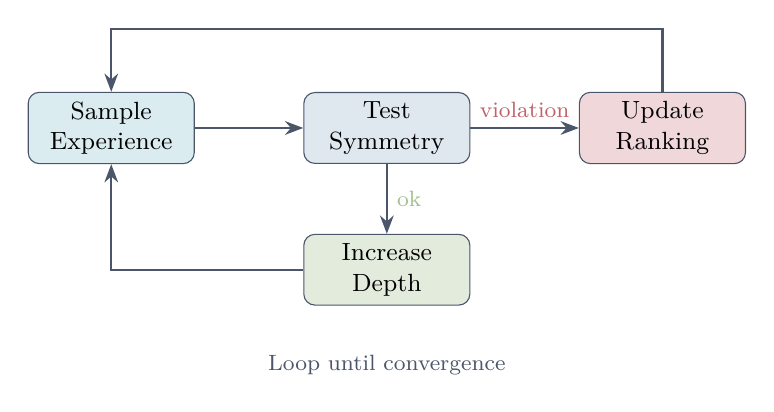
\begin{tikzpicture}[
    node distance=2cm,
    box/.style={draw=nord3,rounded corners,minimum height=2.5em,minimum width=6em,align=center,font=\small,fill=nord5},
    arr/.style={->,thick,>=Stealth,nord3}
]
\node[box,fill=nord8!30] (sample) {Sample\\Experience};
\node[box,fill=nord9!25] (test) at (3.5,0) {Test\\Symmetry};
\node[box,fill=nord11!25] (update) at (7,0) {Update\\Ranking};
\node[box,fill=nord14!30] (refine) at (3.5,-1.8) {Increase\\Depth};

\draw[arr] (sample) -- (test);
\draw[arr] (test) -- node[above,font=\footnotesize,color=nord11] {violation} (update);
\draw[arr] (update.north) -- ++(0,0.8) -| (sample.north);
\draw[arr] (test) -- node[right,font=\footnotesize,color=nord14] {ok} (refine);
\draw[arr] (refine) -| (sample);

\node[below=2.3cm of test,font=\footnotesize,color=nord3] {Loop until convergence};
\end{tikzpicture}
\caption{The learning loop: sample, test for violations, update ranking, refine depth.}
\label{fig:learning-loop}
\end{figure}

\subsection{Violations and Swaps}

Suppose the current ranking at some state is $[\text{Stay}, \text{Go}]$ (Stay preferred), but the Finder discovers at depth~$k$ that Go's trace dominates Stay's.  This is a \textbf{violation}: the ranking disagrees with the evidence.  The fix is to swap Go ahead of Stay, producing $[\text{Go}, \text{Stay}]$.  Each swap fixes exactly one violated pair without disturbing unrelated pairs.

Formally, a violation records which state, which two actions, and at what depth the disagreement was found:

\begin{code}[hide]
module LearningBase
  (State Action : Set)
  (_≟ₐ_ : ∀ (a b : Action) → Dec (a ≡ b))
  where

  open import Data.Bool using (Bool; true; false; if_then_else_; not; _∧_)
  open import Data.Nat using (ℕ; zero; suc; _+_; _≤_; z≤n; s≤s)
  open import Data.Nat.Properties using (≤-refl; +-mono-≤)
  open import Data.List using (List; []; _∷_; _++_)
  open import Data.Maybe using (Maybe; just; nothing)
  open import Data.Product using (_×_; _,_; ∃; ∃-syntax)
  open import Relation.Binary.PropositionalEquality using (_≡_; refl)
  open import Data.Empty using (⊥)

  ExplicitRanking : Set
  ExplicitRanking = State → List Action
\end{code}

\begin{code}
  record Violation : Set where
    constructor violation
    field
      viol-state  : State
      viol-better : Action
      viol-worse  : Action
      viol-depth  : ℕ

  DominanceOracle : Set
  DominanceOracle = State → Action → Action → Bool
\end{code}

\noindent The \texttt{DominanceOracle} is the ground-truth pairwise comparator---in practice, instantiated by the Finder's trace comparison at the current depth.  The fix is to \textbf{swap} the violated pair in the ranking:

\begin{code}[hide]
  is-dominated-by : List Action → Action → Action → Bool
  is-dominated-by [] _ _ = true
  is-dominated-by (x ∷ xs) a b with a ≟ₐ x | b ≟ₐ x
  ... | yes _ | yes _ = true
  ... | yes _ | no  _ = false
  ... | no  _ | yes _ = true
  ... | no  _ | no  _ = is-dominated-by xs a b

  remove-action : Action → List Action → List Action
  remove-action _ [] = []
  remove-action a (x ∷ xs) with x ≟ₐ a
  ... | yes _ = xs
  ... | no  _ = x ∷ remove-action a xs
\end{code}

\begin{code}
  swap-in-list : Action → Action → List Action → List Action
  swap-in-list _ _ [] = []
  swap-in-list better worse (x ∷ xs) with x ≟ₐ worse
  ... | yes _ = better ∷ worse ∷ remove-action better xs
  ... | no  _ = x ∷ swap-in-list better worse xs

  global-swap-updater : Violation → ExplicitRanking → ExplicitRanking
  global-swap-updater v ranking s = 
    swap-in-list (Violation.viol-better v) (Violation.viol-worse v) (ranking s)
\end{code}

\subsection{Monotonicity Guarantee}

The critical question is: does repeated swapping converge?  The answer is yes, and we can bound the number of steps.  The argument has three parts:

\begin{theorem}[Swap Monotonicity]
Let $v$ be a violation with actions $(better, worse)$. After swapping:
(1)~the violated pair is correctly ordered;
(2)~unrelated pairs are unchanged;
(3)~total violations decrease by at least~$1$.
\end{theorem}

\noindent In Agda, part~(1) is \texttt{SwapFixesPair}: after swapping, the oracle confirms the pair is correctly ordered.  Part~(2) is \texttt{SwapPreservesUnrelated}: for any pair $(a, b)$ where neither $a$ nor $b$ is involved in the swap, their relative order is unchanged.  Together, these guarantee that each swap reduces the violation count by exactly one without introducing new violations.

\begin{code}
  SwapFixesPair : Set
  SwapFixesPair = ∀ (better worse : Action) (xs : List Action) →
    (better ≡ worse → ⊥) →
    is-dominated-by (swap-in-list better worse xs) worse better ≡ true

  SwapPreservesUnrelated : Set
  SwapPreservesUnrelated = ∀ (better worse a b : Action) (xs : List Action) →
    (a ≡ better → ⊥) → (a ≡ worse → ⊥) →
    (b ≡ better → ⊥) → (b ≡ worse → ⊥) →
    is-dominated-by xs a b ≡ is-dominated-by (swap-in-list better worse xs) a b
\end{code}

\noindent Since each swap strictly decreases the violation count and violations are non-negative, the process terminates.  The worst case is when every pair at every state is initially violated, giving a convergence bound:
\[
\text{max-violations} \leq |S| \times \binom{|A|}{2} = |S| \times \frac{|A|(|A|-1)}{2}
\]

\begin{code}[hide]
  count-violations-at : ExplicitRanking → DominanceOracle → State → ℕ
  count-violations-at ranking oracle s = count-list (ranking s)
    where
      count-list : List Action → ℕ
      count-list [] = 0
      count-list (_ ∷ []) = 0
      count-list (a ∷ b ∷ rest) = 
        let ranking-says = is-dominated-by (ranking s) a b
            oracle-says  = oracle s a b
            this-viol    = if ranking-says ∧ not oracle-says then 1 else 0
        in this-viol + count-list (b ∷ rest)

  count-total-violations : ExplicitRanking → DominanceOracle → List State → ℕ
  count-total-violations _ _ [] = 0
  count-total-violations ranking oracle (s ∷ ss) = 
    count-violations-at ranking oracle s + count-total-violations ranking oracle ss

  open import Data.Maybe using (Maybe; just; nothing)
  open import Data.Bool using (Bool; true; false)

  iterated-update : (ExplicitRanking → Maybe Violation) → 
                    ExplicitRanking → ℕ → ExplicitRanking
  iterated-update _ r zero = r
  iterated-update find r (suc n) with find r
  ... | nothing = r
  ... | just v  = iterated-update find (global-swap-updater v r) n

  FindViolValid : (ExplicitRanking → Maybe Violation) → Set
  FindViolValid find = ∀ r v → find r ≡ just v → 
    is-dominated-by (r (Violation.viol-state v)) 
      (Violation.viol-better v) (Violation.viol-worse v) ≡ true

  StrictDecrease : DominanceOracle → List State → Set
  StrictDecrease oracle states = ∀ v ranking →
    oracle (Violation.viol-state v) (Violation.viol-better v) 
           (Violation.viol-worse v) ≡ true →
    is-dominated-by (ranking (Violation.viol-state v)) 
      (Violation.viol-better v) (Violation.viol-worse v) ≡ true →
    let swapped = global-swap-updater v ranking
    in suc (count-total-violations swapped oracle states) ≤ 
       count-total-violations ranking oracle states
\end{code}

\noindent The \texttt{ConvergenceTheorem} packages the full guarantee: given a valid violation finder and a ground-truth oracle, iterated swapping from any initial ranking reaches zero violations in at most \texttt{max-violations} steps.  Reading the type: the hypotheses require (i)~\texttt{StrictDecrease}---each swap reduces the count; (ii)~\texttt{FindViolValid}---the finder only reports genuine violations; (iii)~oracle soundness---reported better actions truly dominate; and (iv)~completeness---when no violation is found, the count is zero.

\begin{code}
  ConvergenceTheorem : DominanceOracle → List State → Set
  ConvergenceTheorem oracle all-states = 
    StrictDecrease oracle all-states →
    ∀ (ranking₀ : ExplicitRanking) 
      (find-viol : ExplicitRanking → Maybe Violation) →
    FindViolValid find-viol →
    (∀ r v → find-viol r ≡ just v → 
       oracle (Violation.viol-state v) (Violation.viol-better v) 
              (Violation.viol-worse v) ≡ true) →
    (∀ r → find-viol r ≡ nothing → 
       count-total-violations r oracle all-states ≡ 0) →
    ∃[ n ] (n ≤ count-total-violations ranking₀ oracle all-states × 
            count-total-violations (iterated-update find-viol ranking₀ n) 
              oracle all-states ≡ 0)
\end{code}

\noindent Learning is guaranteed to converge in at most \texttt{max-violations} swaps.  Full proofs are in \fpath{src/CSHRL/Learning/Base.agda}.

\begin{remark}[Full-ranking learning dissolves the exploration/exploitation trade-off]\label{rem:exploration}
The convergence bound $|S| \times \binom{|A|}{2}$ counts \emph{all} pairwise violations, including those between the two worst actions.  To reach zero violations the learner must correctly order every pair---not just identify the argmax.  Uniform pairwise sampling suffices for convergence; no separate exploration mechanism ($\epsilon$-greedy, entropy bonus, UCB) is needed.
\end{remark}

\subsection{Practical Learning Interface}

The learning infrastructure provides a stateful interface supporting:

\begin{itemize}
\item \textbf{Checkpointing:} The \texttt{LearnerState} captures training progress; save to pause, resume by passing to \texttt{train-step}.
\item \textbf{Incremental learning:} Process samples one at a time or in batches.
\item \textbf{Active refinement:} The \texttt{ActiveLearner} maintains an explicit ranking updated on violation (swap), rather than re-querying the Finder.
\item \textbf{Policy materialization:} A \texttt{PolicyTable} is a concrete list of (state, action-ranking) pairs---the verified analogue of trained weights.  At deployment, \texttt{lookup} retrieves the cached ranking in $O(n)$; for states not in the table a fallback to the Finder guarantees no state is ever unhandled.
\end{itemize}

\noindent The same learning loop applies to both CoinductiveHomomorphism and CoindHomo: the only difference is whether the dominance oracle compares successor-value traces or action-value traces.

The output of this learning process is a \emph{total ranking} at every state: every action has a definite position.  This totality is exactly what enables the $O(1)$ adaptation described next---when an action becomes unavailable, we simply skip it in the ranking and pick the next one, with no recomputation needed.

\subsection{Stochastic and Placement Learning}

The learning infrastructure extends to both stochastic MDPs (comparing expected traces; module in \fpath{src/CSHRL/Learning/StochasticFiniteMDP.agda}) and \texttt{CombinatorialPlacementMDP} (short-circuit traces for absorbing Dead/Solved states; module in \fpath{src/CSHRL/Learning/CombinatorialPlacementMDP.agda}).  All monotonicity guarantees carry over.

\section{Instant Adaptation to Action Unavailability}\label{sec:adaptation}

In many practical settings---robotics, network routing, game playing---actions become unavailable at runtime.  Classical RL stores only the argmax action and must recompute the policy at cost~$O(|S| \cdot |A|)$ or worse.

Because the framework maintains a \emph{total ranking} over all actions, adaptation is $O(1)$: when the top-ranked action becomes unavailable, the second-ranked action is already known.

\begin{theorem}[Restricted Preservation]
If ranking $R$ satisfies the homomorphism property for actions $\mathcal{A}$, and $\mathcal{A}' \subseteq \mathcal{A}$ is the set of available actions, then the restriction $R|_{\mathcal{A}'}$ satisfies the same property for $\mathcal{A}'$.
\end{theorem}

\noindent The preservation property is pairwise: the fact that $a \le_a b$ implies stream dominance does not depend on which other actions exist.  Removing unavailable actions leaves the relative order of remaining actions unchanged.

\begin{code}
  Available : Set
  Available = Action → Bool

  filter-available : Available → List Action → List Action
  filter-available _ []       = []
  filter-available p (x ∷ xs) = 
    if p x then x ∷ filter-available p xs else filter-available p xs

  restricted-explicit-ranking : Available → ExplicitRanking → ExplicitRanking
  restricted-explicit-ranking avail ranking s = filter-available avail (ranking s)
\end{code}

\noindent Beyond filtering, actions can be \textbf{demoted} rather than removed---pushed to the end of the ranking so they are used only as a last resort:

\begin{code}
  filter-bool : (Action → Bool) → List Action → List Action
  filter-bool _ [] = []
  filter-bool p (x ∷ xs) =
    if p x then x ∷ filter-bool p xs else filter-bool p xs

  demote-unavailable : Available → List Action → List Action
  demote-unavailable avail xs = available ++ unavailable
    where
      available   = filter-bool avail xs
      unavailable = filter-bool (λ a → not (avail a)) xs
\end{code}

\begin{code}[hide]
  demote-to-end : Action → List Action → List Action
  demote-to-end a xs = filter-bool (λ x → not (is-eq x)) xs ++ kept
    where
      is-eq : Action → Bool
      is-eq x with x ≟ₐ a
      ... | yes _ = true
      ... | no  _ = false
      kept = filter-bool is-eq xs
\end{code}

\begin{code}
  make-action-unavailable : Action → ExplicitRanking → ExplicitRanking
  make-action-unavailable forbidden ranking s = demote-to-end forbidden (ranking s)
\end{code}

\noindent Classical RL stores only the argmax; when that action fails, the policy must be recomputed at cost~$O(|S| \cdot |A|)$.  The framework stores a total ranking, so when the top action fails the second-best is already available---$O(1)$ lookup.

This applies to both conditions: CoinductiveHomomorphism's successor-value preservation and CoindHomo's action-value preservation are both pairwise properties that restrict without loss.

\section{Scope, Assumptions, and Limits}

It is important to distinguish the \emph{coinductive ideal} from the \emph{algorithmic machinery}:
\begin{itemize}
\item \textbf{Coinductive optimality (ideal):} The definitions in \S\ref{sec:agda-core} are about infinite streams and pointwise dominance at every time step.
\item \textbf{Finder (approximation):} The Finder (\S\ref{sec:finder}) compares \emph{finite} traces lexicographically at a fixed depth.  It becomes exact under conditions verified by the Environment Class infrastructure (e.g., horizon sufficiency for placement problems).
\item \textbf{Learner (policy discovery):} The Learner (\S\ref{sec:learning}) wraps Finder-style comparisons into a stateful learning loop.
\end{itemize}

The deterministic framework assumes: finite action space, deterministic step function, decidable reward order, and a horizon parameter for Finder approximation.  Section~\ref{sec:stochastic} lifts to stochastic environments; Section~\ref{sec:abstraction} lifts to infinite state spaces.

A natural objection: the coinductive homomorphism is undecidable in general.  We view this as analogous to AIXI \cite{Hutter2005}: an uncomputable ideal that organizes a hierarchy of practical approximations.  Crucially, Level~$\omega$ (the full coinductive homomorphism) \emph{is} achievable for structured domains: the 8-Queens instance attains it by exploiting binary reward structure and finite game depth.

\section{Verified Instantiations: From Theory to Tasks}

The examples in this section validate that the formal machinery instantiates correctly.  Each one that type-checks is a proof that the framework applies to that task class.

\subsection{TwoState: Minimal Working Example}

\begin{code}
module TwoStateExample where
  open import Data.Nat using (_≤_; z≤n; s≤s)
  open import Data.Nat.Properties using (≤-refl)

  data TwoState : Set where
    Start : TwoState
    Goal  : TwoState

  data TwoAction : Set where
    Go   : TwoAction
    Stay : TwoAction

  two-step : TwoState → TwoAction → TwoState × ℕ
  two-step Start Go   = (Goal , 1)
  two-step Start Stay = (Start , 0)
  two-step Goal  _    = (Goal , 1)

  two-actions : List TwoAction
  two-actions = Go ∷ Stay ∷ []

  open Core TwoState TwoAction ℕ two-step _≤_ _⊔_ 0 two-actions
\end{code}

\noindent At \texttt{Start}, \texttt{Go}'s future is $(1, 1, 1, \ldots)$ and \texttt{Stay}'s is $(0, 0, 0, \ldots)$; the ranking \texttt{[Go, Stay]} satisfies both CoinductiveHomomorphism and CoindHomo (the conditions coincide here since the immediate rewards are aligned).  Full preservation proof in \fpath{src/CSHRL/Tasks/Verified/TwoState.agda}, with no postulates.

\subsection{Delayed Gratification: Depth-Discovery}

\begin{code}[hide]
module DelayedGratificationExample where
  open import Data.Nat using (ℕ; zero; suc; _≤_; _⊔_)
  open import Data.List using (List; _∷_; [])
  open import Data.Product using (_×_; _,_)
  open import Relation.Binary.PropositionalEquality using (_≡_; refl)
\end{code}
\begin{code}
  data DGState : Set where
    Start : DGState
    PathA : DGState
    PathB : DGState
    End   : DGState

  data DGAction : Set where
    GoA  : DGAction
    GoB  : DGAction
    Wait : DGAction

  dg-step : DGState → DGAction → DGState × ℕ
  dg-step Start GoA = (PathA , 0)
  dg-step Start GoB = (PathB , 0)
  dg-step PathA _   = (PathA , 0)
  dg-step PathB _   = (End , 1)
  dg-step End   _   = (End , 1)
  dg-step _     _   = (End , 0)

  all-actions : List DGAction
  all-actions = GoA ∷ GoB ∷ []

  open Core DGState DGAction ℕ dg-step _≤_ _⊔_ 0 all-actions
\end{code}

\noindent At depth~1 both actions yield trace~$[0]$---indistinguishable.  At depth~2 the traces diverge: \texttt{GoA}~$\to [0,0]$, \texttt{GoB}~$\to [0,1]$.  The conditions again coincide (equal immediate rewards).  Full implementation in \fpath{src/CSHRL/Tasks/Classic/DelayedGratification.agda}.

A complementary example is \textbf{Trap Sparse}: three actions at Start, one of which leads to a terminal reward via a trap state.  Unlike Delayed Gratification, the discriminating action has a \emph{different} immediate reward, so depth~1 suffices.  Full implementation in \fpath{src/CSHRL/Tasks/Classic/TrapSparse.agda}.

\begin{figure}[H]
\centering
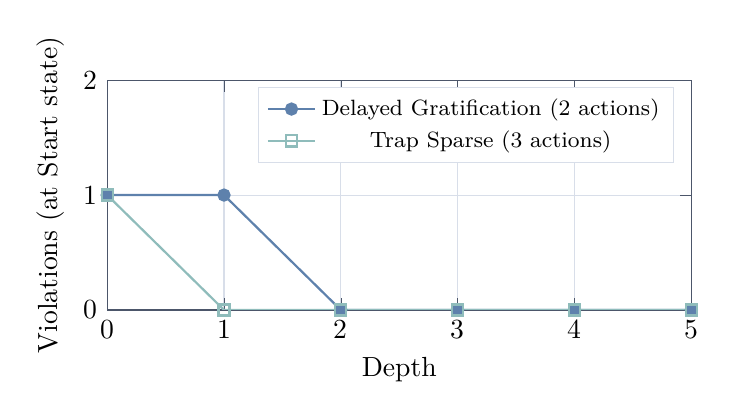
\begin{tikzpicture}
\begin{axis}[
    width=9cm,height=4.5cm,
    xlabel={Depth},
    ylabel={Violations (at Start state)},
    ymin=0,ymax=2,
    xmin=0,xmax=5,
    xtick={0,1,2,3,4,5},
    ytick={0,1,2},
    grid=major,
    grid style={nord4,thin},
    axis line style={nord3},
    tick style={nord3},
    legend pos=north east,
    legend style={font=\footnotesize,draw=nord4}
]
\addplot[thick,mark=*,nord10] coordinates {(0,1) (1,1) (2,0) (3,0) (4,0) (5,0)};
\addlegendentry{Delayed Gratification (2 actions)}
\addplot[thick,mark=square,nord7] coordinates {(0,1) (1,0) (2,0) (3,0) (4,0) (5,0)};
\addlegendentry{Trap Sparse (3 actions)}
\end{axis}
\end{tikzpicture}
\caption{Violations at Start state drop to zero as depth increases.  Delayed Gratification requires depth~2 to distinguish equal-immediate-reward paths; Trap Sparse resolves at depth~1.  Both are verified in \protect\fpath{src/CSHRL/Tasks/Classic/}.}
\label{fig:violations}
\end{figure}

\subsection{Key-Door-Treasure: State-Dependent Rankings}

A robot must collect a key, unlock a door, then reach treasure.

\begin{figure}[H]
\centering
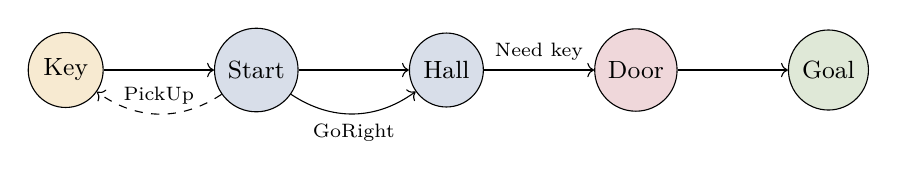
\begin{tikzpicture}[node distance=1.4cm]
  \node[draw,circle,fill=nord13!40,font=\small] (key) {Key};
  \node[draw,circle,right=of key,fill=nord4,font=\small] (start) {Start};
  \node[draw,circle,right=of start,fill=nord4,font=\small] (hall) {Hall};
  \node[draw,circle,right=of hall,fill=nord11!25,font=\small] (door) {Door};
  \node[draw,circle,right=of door,fill=nord14!35,font=\small] (Goal) {Goal};
  \draw[->] (key) -- (start);
  \draw[->] (start) -- (hall);
  \draw[->] (hall) -- (door) node[midway,above,font=\scriptsize] {Need key};
  \draw[->] (door) -- (Goal);
  \draw[->,dashed,bend left=35] (start) to node[above,font=\scriptsize] {PickUp} (key);
  \draw[->,bend right=35] (start) to node[below,font=\scriptsize] {GoRight} (hall);
\end{tikzpicture}
\caption{Key--Door--Treasure: the optimal action depends on whether the key is held.}
\label{fig:key-door}
\end{figure}

\noindent This demonstrates \emph{state-dependent} rankings and the ``ranking flip'' phenomenon:

\begin{center}
\small
\begin{tabular}{l|l|l}
\textbf{State} & \textbf{Without Key} & \textbf{With Key} \\
\hline
Start & [PickUp, GoRight, GoLeft] & [GoRight, GoLeft, PickUp] \\
Hall  & [GoLeft, GoRight, Wait] & [GoRight, Wait, GoLeft] \\
\end{tabular}
\end{center}

The moment the key is acquired, the ranking inverts---a phase transition encoded directly in the traces rather than via gradual value propagation:
\begin{itemize}
\item Without key: \texttt{GoRight} $\to$ $[0, 0, 0, \ldots]$ (blocked)
\item With key: \texttt{GoRight} $\to$ $[0, 0, 100, 100, \ldots]$ (treasure)
\end{itemize}

\begin{sloppypar}
\noindent This validates that state-dependent rankings instantiate correctly under the \texttt{FiniteDeterministicMDP} environment class.  The conditions coincide for this environment (uniform step costs).  Full implementation in \fpath{src/CSHRL/Tasks/Classic/KeyDoor.agda}.
\end{sloppypar}

\subsection{8-Queens: Scalable Verification}

The \texttt{Queens8Learning} module validates the full pipeline end-to-end: learning via \texttt{materialize-on-path} from the empty board, producing a \texttt{PolicyTable} of eight entries.  The following extract illustrates the interface; the full verified instantiation is in \fpath{src/CSHRL/Tasks/Verified/Queens8.agda}.

\begin{code}[hide]
  module Queens8LearningResult where
    open import Data.Nat using (ℕ)
    open import Data.List using (List; _∷_; [])
    open import Data.Product using (_×_)
    open import Relation.Binary.PropositionalEquality using (_≡_; refl)

    data Q8Action : Set where
      C0 C1 C2 C3 C4 C5 C6 C7 : Q8Action

    data Q8State : Set where
      Ongoing : List ℕ → Q8State
      Dead : Q8State
      Solved : List ℕ → Q8State

    PolicyTable : Set
    PolicyTable = List (Q8State × List Q8Action)

    policy : PolicyTable
    policy = []

    horizon : ℕ
    horizon = 8

    run-policy : PolicyTable → ℕ → Q8State → ℕ → List Q8Action
    run-policy _ _ _ _ = C0 ∷ C4 ∷ C7 ∷ C5 ∷ C2 ∷ C6 ∷ C1 ∷ C3 ∷ []
  open Queens8LearningResult
\end{code}

\begin{code}
  test-solution : run-policy policy horizon (Ongoing []) horizon
                ≡ C0 ∷ C4 ∷ C7 ∷ C5 ∷ C2 ∷ C6 ∷ C1 ∷ C3 ∷ []
  test-solution = refl
\end{code}

\noindent This confirms the materialized policy produces a valid non-attacking $8$-Queens placement---verified end-to-end in Agda with \texttt{--safe} and zero postulates.

\subsection{The Sacrifice Environments: Where the Conditions Separate}

The three environments from Section~\ref{sec:strict-generality}---BinarySacrifice, SkillInvestment, and PreparationDilemma---are the verified instantiations that \emph{separate} the two conditions.  Each has a machine-checked CoinductiveHomomorphism proof and a machine-checked proof that no CoindHomo can rank the sacrificing actions.  These live in \fpath{src/CSHRL/Tasks/Verified/BinarySacrifice.agda}, \fpath{src/CSHRL/Tasks/Verified/SkillInvestment.agda}, and \fpath{src/CSHRL/Tasks/Verified/PreparationDilemma.agda}.

\section{Related Work}

The framework connects to multiple research traditions but makes a distinct move: replacing scalar aggregation with a coinductive order on infinite futures, and distinguishing strategic evaluation (CoinductiveHomomorphism) from tactical evaluation (CoindHomo).

\begin{table}[H]
\centering
\small
\renewcommand{\arraystretch}{1.2}
\begin{tabularx}{\textwidth}{|>{\raggedright\arraybackslash}p{0.20\textwidth}|>{\raggedright\arraybackslash}X|>{\raggedright\arraybackslash}X|}
\hline
\textbf{Approach} & \textbf{Core idea} & \textbf{Relationship} \\
\hline
\textbf{Classical RL} \cite{Sutton2018} & Optimize $\sum_t \gamma^t r_t$ via Bellman equations & CoindHomo \emph{subsumes} this; CoinductiveHomomorphism subsumes successor return (\S\ref{sec:subsumes}) \\
\hline
\textbf{Policy Gradients} \cite{Williams1992} & Gradient ascent on expected return & Optimization \emph{method}; our framework defines the \emph{target} \\
\hline
\textbf{Max-Entropy RL} \cite{Haarnoja2018} & Entropy bonus for exploration & Full-ranking objective dissolves exploration/exploitation (Remark~\ref{rem:exploration}) \\
\hline
\textbf{AIXI} \cite{Hutter2005} & Universal prior over computable environments & Both are ideals; ours is \emph{structurally} defined \\
\hline
\textbf{Coalgebra} \cite{Rutten2000} & Infinite behaviors via coinductive definitions & Direct inspiration: $\le_s$ is a coinductive relation \\
\hline
\textbf{MDP Homomorphisms} \cite{vanderPol2020} & Exploit state/action symmetries for efficiency & Complementary: we use order-preservation, not group automorphisms \\
\hline
\textbf{Giry Monad} \cite{Giry1982} & Probability distributions as monad & Direct application: stochastic extension (\S\ref{sec:stochastic}) \\
\hline
\textbf{CertRL} \cite{Vajjha2021} & Coq-verified RL convergence & Complementary: they verify classical RL; we verify coinductive structure \\
\hline
\end{tabularx}
\end{table}

\subsection{Lexicographic Multi-Objective RL}

The most closely related line of work is \textbf{lexicographic multi-objective RL} (LMORL) \cite{Skalse2022,Tercan2024}.  LMORL orders \emph{objectives} (different reward signals) lexicographically.  Our framework orders \emph{timesteps}: the same reward signal is compared pointwise at $t=0$, then $t=1$, then $t=2$, forever.

\begin{itemize}
\item LMORL: ``Safety reward first, then efficiency reward.''
\item Our framework: ``At every moment $t$, the better action's future dominates.''
\end{itemize}

\subsection{The Sacrifice Pattern in RL}

The sacrifice pattern---accepting immediate cost for long-term benefit---is well-known but typically handled by increasing $\gamma$ or via reward shaping.  Our framework is the first to formally decouple optimality from immediate reward via a coinductive condition.  CoinductiveHomomorphism judges actions solely by successor state quality, side-stepping the tension between immediate and future reward that plagues both discounted returns and CoindHomo.

\subsection{Constrained and Safe RL}

Safe RL \cite{Garcia2015} treats some objectives as hard constraints rather than soft trade-offs.  Constrained MDPs optimize a primary reward while ensuring constraint satisfaction (e.g., collision probability~$< \epsilon$).

The framework's relationship to safe RL is complementary:
\begin{itemize}
\item \textbf{Temporal constraints as dominance:} A safety constraint ``never enter state~$X$'' translates to: the safe action's trace dominates at every timestep (the unsafe action's trace eventually shows the penalty).
\item \textbf{No constraint relaxation:} The coinductive order is strict---there is no $\epsilon$-violation.  If $a$'s trace dominates $b$'s at every step, the dominance is absolute.
\end{itemize}

\subsection{Preference-Based, Ordinal, and Ranking RL}

Preference-based RL (PbRL) \cite{Wirth2017} learns from pairwise comparisons rather than scalar rewards.  This connects to our ranking structure, but the relationship is nuanced:
\begin{itemize}
\item PbRL \emph{infers a latent scalar} from comparisons, then optimizes that scalar.  Our framework requires only \emph{ordinal structure}---a partial order on outcomes---and compares streams directly without scalar collapse.
\item The Core module is parameterized by \texttt{\_$\le$ᵣ\_ : Reward $\to$ Reward $\to$ Set}---any partial order suffices.  Human preference orderings are a valid instantiation.
\end{itemize}

\noindent Direct Preference Optimization (DPO) \cite{Rafailov2023} bypasses explicit reward modelling by deriving an implicit scalar reward from pairwise preferences via the Bradley--Terry model, then optimizes a policy to maximize it.  The pairwise structure of the input is discarded once the implicit reward is extracted.  In our framework, by contrast, the pairwise ordering \emph{is} the optimality criterion---preserved coinductively, not collapsed into a scalar.

Deep Ordinal Reinforcement Learning \cite{Zap2019} modifies Q-learning for ordinal rewards via thresholded updates, mitigating overestimation in DQN.  However, it retains discounts and bootstrapping, unlike the coinductive elimination of~$\gamma$.

\subsection{Coalgebraic Foundations}

The coinductive stream order $\le_s$ is a coalgebraic relation in the sense of Rutten \cite{Rutten2000}.  Coalgebra provides the categorical semantics for infinite behaviors, and our formalization directly instantiates these ideas in Agda's guarded coinduction.  The \texttt{coinductive} keyword in the $\le_s$ record is precisely the coalgebraic final coalgebra construction.

MDP homomorphisms \cite{vanderPol2020} exploit state/action symmetries for computational efficiency.  The framework uses a different notion of ``symmetry'': not group-theoretic automorphisms of the state space, but \emph{order-preservation} between rankings and stream dominance.

\subsection{Formal Verification of RL}

CertRL \cite{Vajjha2021} is a Coq library that machine-checks convergence proofs for value and policy iteration on finite MDPs, using the Giry monad for probabilistic reasoning.  While CertRL provides rigorous guarantees for classical tabular RL, our framework extends formal verification to a different paradigm: coinductive structure preservation rather than scalar convergence.  Both projects demonstrate that machine-verified RL theory is feasible; they target complementary foundations.

\subsection{What Distinguishes This Work}

\begin{itemize}
\item \textbf{Criterion vs.\ algorithm:} Classical RL and policy gradients are \emph{algorithms} to optimize a scalar.  Our framework defines an \emph{optimality criterion}---a structural property that rankings may or may not satisfy.
\item \textbf{Temporal structure:} The scalar return $\sum \gamma^t r_t$ erases timing; the coinductive order $\le_s$ preserves it completely.
\item \textbf{Pointwise dominance:} Unlike lexicographic MORL (priority among objectives) or average-reward RL (limit of partial sums), the framework requires dominance at \emph{every} timestep.
\item \textbf{Strategic vs.\ tactical:} CoinductiveHomomorphism judges actions solely by successor state quality; CoindHomo additionally demands immediate reward alignment.  No prior work makes this decomposition.
\item \textbf{Machine verification:} All results are fully implemented in Agda with type-checked proofs.
\end{itemize}

\section{Future Work}

\begin{itemize}
\item \textbf{Continuous distributions:} The stochastic framework (\S\ref{sec:stochastic}) represents distributions as \texttt{List (A $\times$ $\mathbb{N}$)}.  Extending to measure-theoretic distributions would broaden applicability to continuous-outcome environments.
\item \textbf{Continuous action spaces:} The framework assumes finite, enumerable actions.  Extending to continuous action spaces (e.g., torque values) would require replacing enumeration-based ranking with optimization over compact sets.
\item \textbf{Partially observable MDPs:} Lift rankings to belief-state distributions with stochastic transitions.
\item \textbf{Multi-agent settings:} Rankings over joint action spaces with game-theoretic equilibrium conditions.
\item \textbf{Program synthesis as policy representation:} The full-ranking objective (Remark~\ref{rem:exploration}) naturally extends to synthesized programs: a program satisfying all pairwise ranking constraints on observed states encodes sufficient environment structure to generalize to unseen states.
\end{itemize}

\section{Conclusion}

We have presented a framework that redefines optimality as \emph{structure preservation} rather than scalar maximization.  Two coinductive conditions capture two complementary notions of optimality:

\begin{itemize}
\item \textbf{CoinductiveHomomorphism} evaluates actions by the quality of the states they lead to---successor state quality.  It is the strategic condition: an action that sacrifices immediate reward to reach a superior successor is correctly ranked.

\item \textbf{CoindHomo} additionally requires that immediate transition rewards respect the ranking.  It is the tactical condition: the better-ranked action must win both the immediate payoff and the long-term future.
\end{itemize}

\noindent The decomposition theorem establishes their precise relationship: CoindHomo equals CoinductiveHomomorphism plus immediate reward compatibility.  For the vast majority of standard environments, these conditions coincide; three verified counterexamples demonstrate the strict gap.

The framework is supported by machine-verified results in Agda:
\begin{enumerate}
\item \textbf{Subsumption:} Both conditions imply classical argmax optimality for any finite horizon.
\item \textbf{Monotonic learning:} Violation-correction converges in at most $|S| \times \binom{|A|}{2}$ swaps.
\item \textbf{Instant adaptation:} Action unavailability requires $O(1)$ lookup, not full recomputation.
\item \textbf{Stochastic extension:} The framework lifts to probabilistic environments via the Giry monad, with lexicographic coinductive comparison.
\item \textbf{Distributional hierarchy:} FOSD and the SD$[k]$ chain (\S\ref{sec:fosd}--\ref{sec:sd-hierarchy}) give parameterized verification strength for progressively broader utility function classes.
\item \textbf{Compositional algebra:} Verified rankings compose via product, sum, convolution, and scaling.
\item \textbf{State abstraction:} Rankings verified on finite abstract systems lift to arbitrary concrete spaces.
\item \textbf{Scalable verification:} The Environment Class architecture provides automatic trace-to-stream bridges; 8-Queens achieves a full CoindHomo for $8^8$ candidate placements with zero postulates.
\end{enumerate}

\noindent This document is itself the proof: compiling it type-checks all embedded code while producing this PDF.

%%%%%%%%%%%%%%%%%%%%%%%%%%%%%%%%%%%%%%%%%%%%%%%%%%%%%%%%%%%%%%%%%%%%%%%%%%%%%%%
\section{Reproducibility and Build}
%%%%%%%%%%%%%%%%%%%%%%%%%%%%%%%%%%%%%%%%%%%%%%%%%%%%%%%%%%%%%%%%%%%%%%%%%%%%%%%

\begin{itemize}
\item \textbf{Tested toolchain:} Agda 2.7.x, Agda StdLib 2.0, Lua\LaTeX.
\item \textbf{Build commands:} In \texttt{literate/}, run \texttt{make successor} (or \texttt{agda --latex CSHRL-Successor.lagda.tex} followed by \texttt{lualatex}).
\item \textbf{Fonts:} The document uses \texttt{fontspec} and Unicode math fonts (DejaVu, STIX Two Math).
\end{itemize}

%%%%%%%%%%%%%%%%%%%%%%%%%%%%%%%%%%%%%%%%%%%%%%%%%%%%%%%%%%%%%%%%%%%%%%%%%%%%%%%
\begin{thebibliography}{20}

\bibitem{Sutton2018}
Sutton, R.~S. and Barto, A.~G. (2018).
\textit{Reinforcement Learning: An Introduction}, 2nd~ed. MIT Press.

\bibitem{Williams1992}
Williams, R.~J. (1992).
Simple statistical gradient-following algorithms for connectionist reinforcement learning.
\textit{Machine Learning}, 8(3--4):229--256.

\bibitem{Haarnoja2018}
Haarnoja, T., Zhou, A., Abbeel, P., and Levine, S. (2018).
Soft actor-critic: Off-policy maximum entropy deep reinforcement learning with a stochastic actor.
In \textit{Proceedings of ICML}, pp.~1861--1870.

\bibitem{Hutter2005}
Hutter, M. (2005).
\textit{Universal Artificial Intelligence: Sequential Decisions Based on Algorithmic Probability}. Springer.

\bibitem{Rutten2000}
Rutten, J.~J.~M.~M. (2000).
Universal coalgebra: A theory of systems.
\textit{Theoretical Computer Science}, 249(1):3--80.

\bibitem{vanderPol2020}
van der Pol, E., Worrall, D., van Hoof, H., Oliehoek, F., and Welling, M. (2020).
MDP homomorphic networks: Group symmetries in reinforcement learning.
In \textit{NeurIPS}.

\bibitem{Giry1982}
Giry, M. (1982).
A categorical approach to probability theory.
In \textit{Categorical Aspects of Topology and Analysis}, LNCS vol.~915, pp.~68--85. Springer.

\bibitem{Skalse2022}
Skalse, J., Hammond, L., Griffin, C., and Abate, A. (2022).
Lexicographic multi-objective reinforcement learning.
In \textit{IJCAI}, pp.~3430--3436.

\bibitem{Tercan2024}
Tercan, H. and Prabhu, S. (2024).
Thresholded lexicographic ordered multiobjective reinforcement learning.
In \textit{ECAI}.

\bibitem{Wirth2017}
Wirth, C., Akrour, R., Neumann, G., and F{\"u}rnkranz, J. (2017).
A survey of preference-based reinforcement learning methods.
\textit{JMLR}, 18(136):1--46.

\bibitem{Rafailov2023}
Rafailov, R., Sharma, A., Mitchell, E., Ermon, S., Manning, C.~D., and Finn, C. (2023).
Direct preference optimization: Your language model is secretly a reward model.
In \textit{NeurIPS}.

\bibitem{Vajjha2021}
Vajjha, K., Shinnar, A., Trager, B., Pestun, V., and Fulton, N. (2021).
CertRL: Formalizing convergence proofs for value and policy iteration in Coq.
In \textit{CPP '21: Certified Programs and Proofs}, pp.~18--31. ACM.

\bibitem{Li2006}
Li, L., Walsh, T.~J., and Littman, M.~L. (2006).
Towards a unified theory of state abstraction for MDPs.
In \textit{ISAIM}.

\bibitem{Garcia2015}
Garc{\'\i}a, J. and Fern{\'a}ndez, F. (2015).
A comprehensive survey on safe reinforcement learning.
\textit{JMLR}, 16(42):1437--1480.

\bibitem{Zap2019}
Zap, A., Chaudhuri, S., and Topcu, U. (2019).
Deep ordinal reinforcement learning.
In \textit{AAMAS}, pp.~1838--1846.

\bibitem{Bellman1957}
Bellman, R. (1957).
\textit{Dynamic Programming}.
Princeton University Press.

\bibitem{Watkins1992}
Watkins, C.~J.~C.~H. and Dayan, P. (1992).
Q-learning.
\textit{Machine Learning}, 8(3--4):279--292.

\bibitem{Mnih2015}
Mnih, V., Kavukcuoglu, K., Silver, D., Rusu, A.~A., Veness, J., Bellemare, M.~G., et~al. (2015).
Human-level control through deep reinforcement learning.
\textit{Nature}, 518(7540):529--533.

\end{thebibliography}

\end{document}
